% Created 2019-04-17 Wed 12:42
% Intended LaTeX compiler: pdflatex
\documentclass[a4paper,12pt,twoside,openright]{report}
\usepackage[utf8]{inputenc}
\usepackage[T1]{fontenc}
\usepackage{graphicx}
\usepackage{grffile}
\usepackage{longtable}
\usepackage[acronym]{glossaries}
\usepackage{wrapfig}
\usepackage{rotating}
\usepackage[normalem]{ulem}
\usepackage{amsmath}
\usepackage{textcomp}
% \usepackage{biblatex}
\usepackage{amssymb}
\usepackage{verbatim}
\usepackage{capt-of}
\usepackage[pdfborder={0 0 0}]{hyperref}    % turns references into hyperlinks
\usepackage{docmute}   % only needed to allow inclusion of proposal.tex
\usepackage[margin=25mm]{geometry}
\date{\today}
\title{}
\hypersetup{
 pdfauthor={},
 pdftitle={},
 pdfkeywords={},
 pdfsubject={},
 pdfcreator={Emacs 26.2 (Org mode 9.1.14)},
 pdflang={English}}

\raggedbottom                           % try to avoid widows and orphans
\sloppy
\clubpenalty1000%
\widowpenalty1000%

\renewcommand{\baselinestretch}{1.1}    % adjust line spacing to make
% more readable


\graphicspath{ {figures/} }

\usepackage{biblatex}
\addbibresource{references.bib}

\begin{document}

% Title
%==========================================================

\hfill{\LARGE \bf Andrei-Vlad Bădeliță}

\pagestyle{empty}

\vspace*{60mm}
\begin{center}
\Huge{\bf Implementing Parallelism in Lisp for REDUCE} \\
\vspace*{5mm}
Part II Computer Science Dissertation \\
\vspace*{5mm}
Trinity College \\
\vspace*{5mm}
\today  % today's date
\end{center}

\cleardoublepage

%==============================================

\pagestyle{plain}
\pagenumbering{roman}

\section*{Declaration of originality}

I, Andrei-Vlad Bădeliță of Trinity College, being a candidate for Part II of the
Computer Science Tripos, hereby declare that this dissertation and the work described
in it are my own work, unaided except as may be specified below, and that the
dissertation does not contain material that has already been used to any
substantial extent for a comparable purpose.

\medskip
\noindent
I, Andrei-Vlad Bădeliță of Trinity College, am content for my dissertation
to be made available to the students and staff of the University.

\bigskip
\leftline{Signed [signature]}

\medskip
\leftline{Date [date]}

\section*{Proforma}

{\large
\begin{tabular}{ll}
Candidate Number:   & \bf [Candidate No.] \\
Project Title:      & \bf Implementing Parallelism in Lisp for REDUCE \\
Examination:        & \bf Computer Science Tripos -- Part II, 2019  \\
Word Count:         & \bf 9830        \\
Final code line count: & \bf 8803        \\
Project Originator: & Dr. Arthur C. Norman                    \\
Supervisor:         & Dr. Arthur C. Norman                    \\
\end{tabular}
}

\subsection*{Original Aims of the Project}

To implement a multi-threaded version of a Lisp interpreter. It should
allow the user to create threads and offer the primitives necessary to
write parallel programs. The original language is able to build and
run a complete computer algebra system, which the parallel version should
be able replicate fully. Additionally, a number of tests and algorithms will
be implemented to evaluate correctness and the potential benefits of parallelism.

\subsection*{Work Completed}

All of the original goals have been achieved. The multi-threaded Lisp
is showing predictable speed-ups when executing tasks in parallel,
while preserving full backwards compatibility with the original language.

\subsection*{Special Difficulties}
There were no special difficulties encountered.

\newpage

\setcounter{tocdepth}{2}
\tableofcontents

\newpage

% Chapters
%=============================================================

\pagestyle{headings}

\setcounter{page}{0}
\pagenumbering{arabic}

\chapter{Introduction}
The motivation for this project is to explore the implementation of multi-threading
capabilities within a working compiler and assess the benefits and trade-offs it brings
to a real-world application with a large, actively-developed body of code.

\section{Reduce}

Reduce \cite{reduce} is a portable general-purpose computer algebra system (CAS). It enables symbolic
manipulation of mathematical expressions and provides a wide range of algorithms
to solve problems spanning many fields, with arbitrary precision numerical approximation.
It has a friendly user interface and can display maths and generate graphics.

Reduce is one of a few open-source general-purpose CAS programs, alongside Maxima and Axiom.
The three projects are all built on top of different Lisp kernels. At the time of this writing,
none of these projects have any multi-threaded capabilities. My aim is to remove this limitation
for Reduce. The project is using its own Lisp dialect which is similar to Common Lisp, but has its
own design and set of capabilities.

\section{VSL}

There are multiple implementations of the Lisp backend Reduce uses: PSL, CSL and VSL.
Visual Standard Lisp (VSL) is an interpreted language written
in \texttt{C}. It is fully capable of building the entirety of Reduce, supports all the major
platforms and architectures, and is well optimised for speed, minimising the performance tradeoff
of being interpreted. It exists to provide a test-bed for ideas that may later move to the much larger,
compiled CSL version.

\section{Benefits of multithreading}
The idea of using parallel computing to speed up computer algebra computing has come
up in research papers for many years \cite{GabrielQML,multilisp,multilisp-implementation},
but much of the activity
pre-dates the now ubiquitous multi-core CPUs used in modern computers and the amount of memory
they now provide. Moreover, advancements in single-core CPU performance has slowed down
significantly, as clock speeds have stagnated and even gone down in recent years. The biggest
area of improvement in these new CPUs is their core count and number of hardware threads.
Binding the performance of Reduce to single-threaded performance is likely to lead to
a limitation in speed gains from new hardware. This project involves proving the infrastructure
Reduce will need to take full advantage of today's hardware.

\section{Code examples}

To help explain the concepts I introduce, I will use code fragments to show the algorithms.
These fragments will be a simplification of the original code, in order to remove the need
for context within the rest of the codebase. To that end, the names and function interfaces
are different from the real implementation. More complete versions of the code fragments
I showcase can be found in the Appendix \ref{ch:appendix-code}.

For examples relating to the implementation of the interpreter, I will be using C++.
For work related to my evaluation, I will be showcasing the ParVSL language, which is a type
of Lisp. Reduce implements an additional language running on top of Lisp, called RLisp.
I have tried my best to keep RLisp examples short and as readable
as possible. Where I think the syntax of the language get in the way of readability, I
switch to pseudo-code to aid my explanations.

% TODO: Write Achievements (see Arthur's comments)
% \section{Achievements}
% \label{sec:achievements}

% My project involved modifications to several thousand lines of C/C++ code, upgrading it to
% make better idiomatic use of C++ as well as adding concurrency support. It has also used raw
% Lisp code in bracket notation, along with the

\chapter{Preparation}
\section{ParVSL}
I have forked the original VSL project into a new language which I named Parallel VSL, or ParVSL.
ParVSL is fully backwards compatible with VSL and will be compared against it for performance.

VSL was a good candidate for this project because it featured a complete, working Lisp implementation while being
small enough to be a manageable project. The entire VSL codebase consists of around 10000 lines of code, all of which
was originally contained within a single file. Before making changes in critical areas, I spent some time familiarising
myself with the code. This included splitting the project into multiple files, fixing a few obvious bugs, and porting
from C to C++.

\section{From C to C++}
The VSL language was written in the C programming language. C is a language with no standardised
multi-threaded model and no native support for multi-core programming. Furthermore, it has no well-defined
memory model, and no defined ordering of memory accesses. Multi-threaded programming
is only possible in C through a third-party library, such as \texttt{Windows threads} or the
the \texttt{POSIX threads} library on UNIX systems. Support has to be provided by individual compilers
and operating systems and can break between versions.

C++ is a superset of C and can compile existing, standard C code. The C++11 standard addresses the
above omissions, making C++ a multi-threaded language. While in some cases the implementation uses the same
libraries as the C equivalent (e.g. POSIX), I do not have to think about these details and the code
I write is fully portable. The only requirement is that a C++11 compliant compiler is used supporting
the target platform. As of today, the C++11 standard has matured enough
that all the large compiler vendors (i.e. GCC, Clang, Visual C++, Mingw, etc.) fully support it on the
major platforms (e.g. x86, ARM and SPARC).

The first change I have made to the implementation is to clear it of any incompatible code and compile it
with a C++ compiler. This mostly involved adding a few more explicit casts\footnote{e.g.
C++ is stricter than C about the need for \texttt{const} qualifiers on pointers that
may refer to C-style strings.}.
However, I also transitioned the code to idiomatic C++ as I analysed more parts of it
and became confident those changes wouldn't affect the semantics of the program.

\subsection{RAII classes}
\label{sec:raii}
The \emph{RAII (Resource Allocation Is Initialisation)} design pattern is common in C++ \cite[Item~37]{effective-cpp}.
It is a programming technique which binds the lifetime of resources to an object's lifetime. Normally,
C and C++ are manually managed, meaning all resources have to be carefully tracked by the programmer.
This makes it easy to introduce bugs when there is an attempted access to an unallocated resource,
or leaks when a resource is not released after use. C++ classes offer a solution to this problem.
Classes have both constructors and destructors, and these are automatically called when the object
is created and when it becomes unavailable (it goes out of scope or it is deleted), respectively.

We can use this mechanism to implement RAII. We simply make sure
the underlying resource is allocated in the constructor and deallocated in the destructor.
Smart pointers like \verb|std::unique_ptr| are a good showcase of the power of RAII. As soon as the
smart pointer objects become inaccessible (e.g. by going out of scope), the underlying pointer
is safely deleted, providing a primitive (but very effective) form of automatic reference counting.

When changing the codebase to use C++ features I found various opportunities to apply the RAII pattern:
for managing threads, shallow binding and for garbage collection synchronisation.

\section{Throughput vs latency}
When optimising for performance in a programming language, we have to analyse the trade-off between
total throughput and latency. Optimising for latency means minimising the duration of any individual
task in the program, and increasing availability. Optimising for throughput involves minimising the
total running time of the program.

In a CAS program the user is most likely to care about throughput, i.e. for computing the outputs of large
problem sizes as quickly as possible. The program is single-user and has a simple interface. The only case
for low latency is in the responsiveness of the graphical user interface. This is already provided by the
operating system so our main goal is directed towards maximising throughput in the application.
This is particularly important when designing the garbage collector.

\section{The read-eval-print loop}

The VSL Lisp system has a \emph{read-eval-print} loop at its core: it reads the next instruction, evaluates
it and prints the result. When evaluating performance, I carefully analysed the functions
called within this loop. These functions constitute the \emph{critical path}. The code on the critical
path is the most heavily used and should be as efficient as possible. When I modify it to enable
multi-threading, I pay special attention to not encumber it.

\section{Memory allocation}
Memory is managed by the interpreter. VSL allocates a large block of memory at the beginning,
which it then manages as a contiguous array. When running out of memory, an extra block of the
same size as the one in use is \verb|malloc|-ed, doubling the amount available. These blocks are
never freed until the end of the program. They are sorted by their pointer locations,
and behave as if they were \emph{joined} together to maintain the abstract model of contiguous memory.
Binary search is used to identify the block containing a location.

The allocations are efficient, using a simple pointer, called \emph{fringe} to indicate the start of the
free area of memory. An additional pointer \emph{limit} indicates the end of free memory. To allocate,
VSL checks whether there is enough space, then simply increments the fringe by the specified amount.
If the allocation would cross \verb|limit|, it triggers \emph{garbage collection}.

\begin{figure}[H]
    \centering
    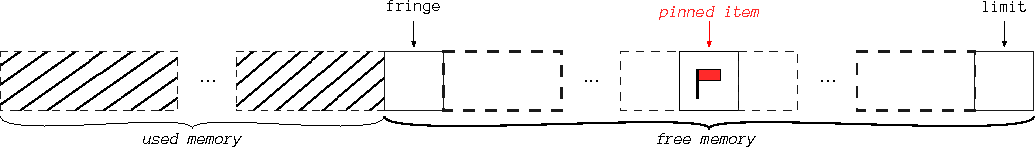
\includegraphics[width=1\linewidth]{vslalloc.pdf}
    \label{fig:vslalloc}
    \caption{Memory allocations in VSL}
\end{figure}

\section{Garbage collector}
An important feature of Lisp languages is the \emph{Garbage Collector} (GC). Garbage collectors allow the programmer
to design code without having to worry about the lifecycle of their data, the internal memory model or
managing pointers. This makes Lisp code significantly easier to write, leaving the burden of providing safety and
efficiency to the system.

In effect, the garbage collector is an important component of VSL and careful considerations
have to be made when modifying it. First of all, any bugs in the garbage collector may leave the memory in
an invalid state, corrupting the state of the program and leading to undefined behaviour in C. Such errors
are also very difficult to spot and debug, as they can go undetected until the particular region of memory
is accessed again.

\subsection{Cheney's algorithm}
The approach a garbage collector uses to deal with freed memory affects both its performance and memory usage.
Before the first garbage collection cycle, memory can simply be allocated in a continuous fashion, making it
compact and fast. When the garbage collector finds unreachable objects and eliminates them, they will leave
\emph{gaps} behind and cause \emph{fragmentation}.

The algorithm is \emph{stop-the-world}:
it requires pausing execution of the program until the entire collection is over.
The alternative, an \emph{incremental} GC would use minor collections which only partially reclaim memory.
Such an algorithm would only reduce latency at the expense of throughput and fragmentation.

Cheney's algorithm \cite{cheney} is a way of implementing a copying garbage collection.
The virtual \emph{heap} is divided into
two halves, and only one half is in use for allocations. The other half is considered free and used during garbage
collection. When the first half is full and garbage collection is triggered, all traceable objects are copied over
to the second half. Then, the two halves are swapped.

To start the tracing we need to consider a \emph{root set}: a subset of objects which are known to be in use.
One example of elements in the root set is the set of symbols that are in use at the start of garbage collection.
The stack also contains pointers to objects and must be scanned when computing the root set.
While these are the main components of the root set, the interpreter may contain others depending on language features
and implementation, all of which must be spotted and added.

Using the root set, we can trace all references to build the reachable set. Objects may contain references
to other objects, which are also considered reachable.
All objects in the reachable set must be kept during collection, while everything else may be safely collected.
Cheney's algorithm copies over the objects in the root set first. It also modifies their original location to become
a \emph{forwarding reference}: a note indicating that they were moved and what their new location is. Then, it scans
the newly allocated memory (the objects copied over) for more references.
For example, a list object will contain a reference to the rest of the list which is now also copied over.

Please refer to appendix \ref{sec:cheneycode} for a more detailed implementation of the algorithm.

\subsection{Conservative GC}

Garbage collection may start in the middle of a large computation and the references on the stack cannot be discarded.
One safe, but slow approach of dealing with this is to keep a virtual stack. Such a stack could be well typed and easily scanned to find
references. Another is to tag all data on the stack with an extra bit indicating which values are pointers. This approach
is used in OCaml \cite[Chapter~20]{rwoc}, yet it still has the disadvantage of limiting integer types and requiring an extra
instruction (i.e. shift) during runtime.

Instead, VSL uses a \emph{conservative} GC, meaning it over-approximates the root set.
It treats all values on the stack as potential references, called \emph{ambiguous} roots.
This means we are overestimating the set of roots. Unlike \emph{unambiguous} roots (like the symbol table above), we
have to be careful when handling these values, and cannot manipulate them as ordinary Lisp objects, which rules out
copying them over. The solution was
to \emph{pin} them, i.e. mark them in the heap so they are not moved. Listing \ref{code:scanpinned}
shows the process of pinning objects.
Any location on our heap which is pointed to by an ambiguous root is pinned and not copied over.
Additionally, the \texttt{allocate} function will have to check for pinned items on the heap and skip over them.
When building the entirety of REDUCE, the number of pinned items does not reach 300.
Considering memory used is in the order of megabytes, these pinned locations cause negligible fragmentation.

\begin{code}
\begin{minted}[breaklines,mathescape]{c++}
int main() {
  ...
  // before starting the Lisp interpreter
  c_stack_base = approximate_stack_pointer();
  ...
}

void garbage_collection() {
  c_stack_head = approximate_stack_pointer();

  // scan the stack from its head to base
  for (uintptr_t s  = c_stack_head;
                 s  < c_stack_base;
                 s  += sizeof(LispObject))
    if (in_heap(s)) { // check if s points to the virtual heap
      set_pinned(s); // found an ambiguous root
    }
  ...
}
\end{minted}
\caption{Scanning the stack before GC for ambiguous references.}
\label{code:scanpinned}
\end{code}

\subsection{Running single-threaded}

I decided to run the garbage collector on a single thread. This approach still requires synchronisation with all running
threads, however it requires no extra inter-locking during collection. Implementing a safe multi-threaded garbage collector
efficiently would probably merit its own project. I believe that for the small hardware thread counts of current day computers
a single threaded algorithm is adequate, not having to deal with data races and inter-locks. However, his may change as
CPU core counts increase.

\section{Symbols and variable lifetime}
As the original language is decades old, its mechanism for variable lifecycle is not in line with that of modern languages.
This mechanism was counter-intuitive at first, and is lacking in providing safety to the user of the language.

There are two lifetime specifiers for \emph{symbols}: \emph{global} and \emph{fluid}. It is important to note that they
do not refer semantically to variables but only to symbol names.

A \emph{global} symbol has only a single globally visible value. That means you cannot bind the name to any local
variable. For instance if \texttt{x} is declared global, it then cannot be used as a function parameter name, or in a
let binding.

A \emph{fluid} variable has a global value, but can also be locally bound. Fluids behave more like globals do
in other languages, allowing the name to be reused.

\texttt{Let} bindings and function parameters introduce \emph{local} symbols. If the symbol name is already declared global,
it will result in an error. If it is a fluid and has a global value, that value will be shadowed for the lifetime
of the binding.

\section{Debugging tools}

Debugging multi-threaded code is especially difficult and I
needed the right tools to help me find the source of issues. I used
the \verb|gdb| \cite{gdb} debugger to step through code and find the source
of the problem. I used \verb|gprof| \cite{gprof} to profile my code and find
the areas on the critical path which needed optimisations the most. Finally,
I used \verb|valgrind| \cite{valgrind} to analyse ParVSL for memory
problems, data races and undefined behaviour.


\chapter{Implementation}
\section{Integrating threads}
\label{sec:babythreads}
After familiarising myself with the VSL codebase I tried to implement the simplest form of
multi-threading and test out how the language would behave. I added a new function called \verb|thread|
to VSL which takes a piece of code as an argument, starts a new thread and joins again with
the main thread. Once implemented, I could run the first and simplest unit test for ParVSL:

\begin{verbatim}
> (dotimes (i 4) (thread '(print "Hello World")))
"Hello World"
"Hello World"
"Value: Hello Worln"Hello Woird"
ld"
\end{verbatim}

We can immediately observe the effects of parallelism in action. The interpreter is not thread-safe and data races
on global variables (including printing to the same stream) lead to undefined behaviour. Although printing
is possible, most other functions would fail. The spawned threads can only handle strings
and will crash on handling numbers or symbols, or when trying to allocate anything.
There is no inter-thread communication or exception safety, and any garbage collection would produce a segmentation
fault. To be able to write a more complicated test, I need to make changes in all areas of the interpreter.

To manage the threads, I made further use of the C++11 standard library. I devised a global hashmap storing
all the running threads. Creating and joining a thread is done under a mutex lock. Each thread is assigned its own unique
identifier, which is returned to the user. Subsequently, the user can then use the identifier to join the thread.

\section{Memory allocation}
\label{sec:malloc}
\label{sec:storage}

I wanted to allow multiple threads in parallel without affecting the performance
of allocations. To do this I had to use a lock-free approach. As such, I further
split the memory into regions, which I call \emph{segments}. A segment is a thread-local region
for allocation on the heap (see figure \ref{fig:parvslalloc}).

Just like before, memory is allocated to the segments in a continuous
fashion. A pointer indicates the start of the non-allocated part of the segment
(the \emph{segment fringe}), while another tells us the end of the segment
(the \emph{segment limit}).

\begin{figure}[H]
  \centering
  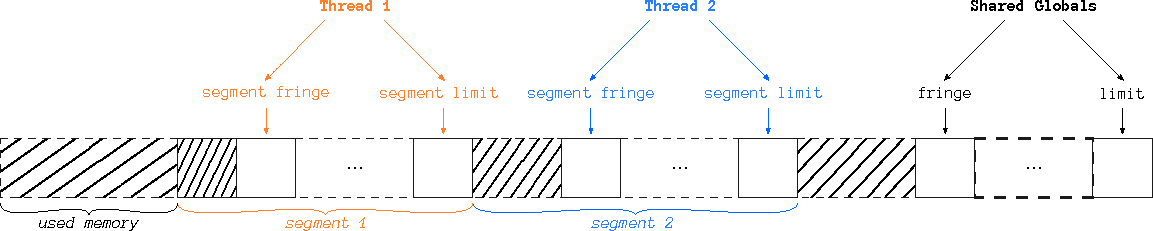
\includegraphics[width=1\linewidth]{parvslalloc.pdf}
  \caption{Memory allocations in ParVSL}
  \label{fig:parvslalloc}
\end{figure}

Now, contention is reduced to getting a new segment. Each thread only allocates within
its own segment, so allocations do not require any synchronisation, and they still only
require incrementing one variable in most cases. If the requested allocation would bring
the segment fringe over the segment limit, then the current segment is \emph{sealed} and a new one is
requested.

I carefully modified all the areas where allocations are performed to use the segment fringe
instead of the global fringe. The global fringe is only moved to assign a new segment. Writes
to the global fringe are executed under a mutex lock, while the segment fringe is a thread local
variable accessed without any locks. If the requested memory is larger than the segment size
(e.g. a large string or number), it is allocated outside any segment, using the global fringe.

There is a trade-off involved when choosing the segment size. If the size is too small,
there will be a lot of contention on requesting segments, leading back to the original
problem of locking on every allocation. If the segment size is too large, there is a risk
of threads holding large amounts of memory without using it and causing internal fragmentation and
early garbage collection cycles. This is because reclaiming memory is requested when a new segment cannot be created,
regardless of how much free space there is in existing segments. While the trade-off depends on the
total memory, I have found a good compromise for segments of a few kilobytes each.

\section{Garbage collection}
\label{sec:gc}
The garbage collector has to account for the state of all threads. These threads have to be synchronised
and in a \emph{safe} state to initiate the GC. They must also be included in the calculation of the root set.

I store all the thread-local information required for synchronisation in a class called \verb|Thread_data|. This
class is populated when a thread is started and updated before and after a GC cycle. All threads register
themselves in a global thread table at start-up. The thread starting the GC can use this table to check the status
of the other threads.

Each thread will have its own stack, so I had to modify the code to scan all the stacks before garbage
collection. This is one reason I had to pause work on all threads for GC. If I didn't it would be possible
for a thread to add references to the heap on its stack after those locations were marked safe to delete,
causing corruption.

When a thread is initialised, I save its own stack base in \verb|Thread_data|, and then also save its stack head
when it is paused to wait for GC. All these stack ranges are scanned before I start garbage collection, as shown
in \ref{code:parstackscan}.

\begin{code}
\begin{minted}[breaklines,mathescape]{c++}
void garbage_collection() {
  for (auto thread: thread_table)
    // scan the stack from its head to base
    for (uintptr_t s = thread.c_stack_head;
                   s < thread.c_stack_base;
                   s += sizeof(LispObject))
      if (in_heap(s)) { // check if s points to the virtual heap
        set_pinned(s); // found an ambiguous root
      }
  ...
}
\end{minted}
\caption{Scan the stack of each thread for pinned items before GC.}
\label{code:parstackscan}
\end{code}

\subsection{Garbage collection locks and safety}
\label{sec:gclock}
The thread initiating garbage collection must wait for all
threads to be ready. Similarly, to prevent starvation, all threads must regularly check
whether a garbage collection cycle was initiated and make themselves safe.

The first idea I had was to trap all calls to allocate memory and check whether garbage collection is needed.
To do this, I could simply reset all thread segments. Threads would need to allocate eventually and
would request a new segment, at which point they would need to call the GC. However, this solution is incomplete:
a thread might be busy for a long time without needing to allocate. This would cause all other
threads to be idle waiting for it to finish.

A bigger issue was the risk of deadlocks. In figure \ref{fig:gcdeadlock}, thread 2 for thread 1 to release
but thread 1 was paused waiting for the GC, causing a deadlock. Similarly, any effectful computation,
like waiting for user input will prevent the collection from starting.

\begin{figure}[H]
  \centering
  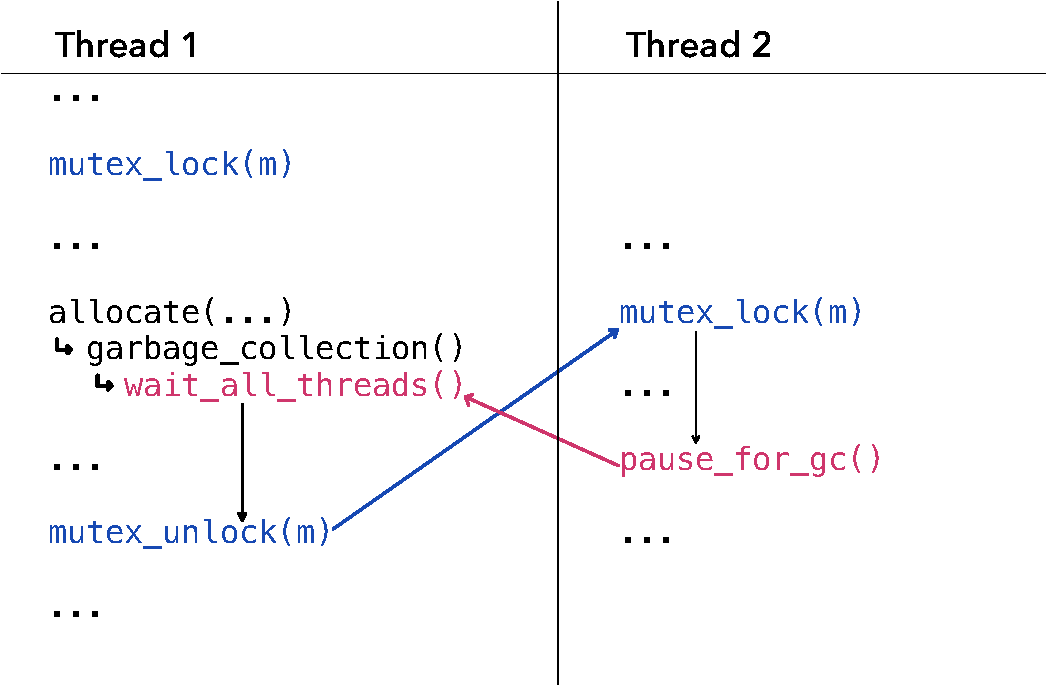
\includegraphics[width=0.8\linewidth]{gcdeadlock.pdf}
  \caption{Possible deadlock when starting garbage collection}
  \label{fig:gcdeadlock}
\end{figure}

I implemented three mechanisms
for a thread to check for garbage collection. The first one is when it tries to allocate. Then, it
polls the global flag in the interpreter, so that time-consuming loops which do not allocate do not
delay the garbage collector for too long. Finall

There are three scenarios in which a thread should check for GC. The first one is when it tries to allocate.
Then, it should poll a global flag in the interpreter, so that time-consuming loops which do not allocate do not
delay the garbage collector for too long. Finally, it must handle any blocking operation, especially
when it depends on a signal from another thread (as in \ref{fig:gcdeadlock}).

I created two classes to help me synchronise threads for GC and handle all the scenarios above:
\verb|Gc_guard| and \verb|Gc_lock|.
To begin with, I used the following shared global state:
\begin{code}
\begin{minted}[breaklines,mathescape]{c++}
  std::atomic_int num_threads(0);

  // number of threads ready for GC
  std::atomic_int safe_threads(0);

  // to wait for all threads to be GC-safe
  std::condition_variable gc_wait_cv;

  // to notify all threads that GC is completed
  std::condition_variable gc_done_cv;

  // flag indicating gc is running (or pending)
  std::atomic_bool gc_on(false);
\end{minted}
\end{code}

To deal with the issue of blocking calls, I defined another state threads can be in: \emph{safe for GC}. A thread
is in a safe state if it has saved all the information the garbage collector needs to begin (e.g. stack base
and stack head) and guarantees not to run any code that invalidates the garbage collection. Threads go into a safe
state whenever they get paused for GC. However, they can also be in safe state when waiting for a blocking call.

The \verb|Gc_guard| class handles both scenarios.
It has a constructor and a destructor and is a way for the thread to promise it is in a safe state.

\begin{code}
\begin{minted}[breaklines,mathescape]{c++}
class Gc_guard {
  // Global mutex shared by Gc_guard instance.
  static std::mutex gc_guard_mutex;

  Gc_guard() {
    td.c_stack_head = approximate_stack_pointer();

    // This thread is now safe for GC.
    safe_threads += 1;

    // Notify the thread waiting for garbage collection.
    gc_wait_cv.notify_one();
  }

  ~Gc_guard() {
    std::unique_lock<std::mutex> lock(gc_guard_mutex);

    // Wait until GC is done.
    gc_done_cv.wait(lock, []() { return !gc_on; });

    // Thread is not longer safe for GC.
    safe_threads -= 1;

    // Thread stack head will be invalidated when execution resumes.
    thread_data.c_stack_head = nullptr;
  }
};
\end{minted}
\caption{\texttt{Gc\_guard} makes a thread safe for GC.}
\label{code:gc-guard}
\end{code}

The \verb|Gc_guard| is designed to be used before any blocking call. For example,
to fix the issue in figure \ref{fig:gcdeadlock}, we simply need to modify the
code in thread 2 as follows:

\begin{code}
\begin{minted}[breaklines,mathescape]{c++}
...
{
  Gc_guard gc_guard; // thread is now safe for GC
  mutex_lock(m); // this operation may block.

  // Gc_guard destructor will block here until GC is completed.
}
...
\end{minted}
\end{code}

The \texttt{Gc\_guard} class is accompanied by \texttt{Gc\_lock}. A thread trying to initiate the GC has to
acquire a \texttt{Gc\_lock}. This lock makes further use of a mutex lock for mutual exclusion.
Additionally, it waits until all threads are in a safe state.

\begin{code}
\begin{minted}[breaklines,mathescape]{c++}
class Gc_lock {
  // Global lock shared by Gc_lock instances.
  static std::mutex gc_lock_mutex;

  // Prevents other threads from acquiring the Gc_lock.
  std::unique_lock<std::mutex> lock;

  // The GC thread needs to be in a safe state as well.
  Gc_guard gc_guard;

  // Initialise the lock and guard before Gc_lock is constructed.
  Gc_lock() : lock(gc_lock_mutex), gc_guard() {
    gc_on = true;

    // Wait until all threads are in a safe state.
    gc_wait_cv.wait(lock, []() {
      return paused_threads == num_threads;
    });
  }

  ~Gc_lock() {
    gc_on = false;

    // Notify all threads that GC is over.
    gc_done_cv.notify_all();
  }
};
\end{minted}
\caption{Garbage collection must be done under the \texttt{Gc\_lock}.}
\label{code:gc-lock}
\end{code}

\section{Lock-free hashtable for symbol lookup}
\label{sec:hashtable}
Just like allocations are a critical region of code in VSL, so are symbol lookups.
Every occurrence of a symbol must be looked up in the symbol table. If the symbol does
not exist, it will be created. Multiple threads looking up symbols will cause contention.
If two threads try to allocate the same symbol name at the same time, they will invalidate
the table.

As before, the na\"ive solution would be to implement a mutex lock on the entire
lookup function.

To improve on that I tried to use a reader-writer lock. Reader-writer locks allow grant access
to either a single writing thread, or all the reading threads. This would allow multiple
threads to lookup symbols at the same time. However, as soon as one one thread has to create a
symbol, all the readers have to wait for it to finish.

Moreover, the lookup function is two-step: first it tries to find a symbol, then it creates one
if it did not find any. In the case of two threads looking up the same symbol, it is possible for
both of them to end try to create it at the same time. The reader-writer lock would not prevent this.
It serialises the writes, so it does prevent undefined behaviour in C++, however it may
still create the same symbol twice. The pointer to the symbol that the first thread returned from the function
would become invalid.

I have found a third approach, based on the Compare-And-Swap (CAS) instruction which solves the issue
above, while also providing a lock-free implementation. The symbol lookup table is currently implemented
as a static array of linked lists. VSL never erases symbols, which made the lock-free implementation easier.

\begin{code}
\begin{minted}[breaklines,mathescape]{c++}
std::atomic<LispObject> symbol_table[TABLE_SIZE];

LispObject lookup(std::string name) {
  size_t loc = hash(name) % SYMBOLS_SIZE;

  LispObject bucket = symbols[loc].load(std::memory_order_acquire);

  while (bucket != nil) {
    LispObject s = head(bucket); // first list element

    if (symbol_name(s) == name) {
      // found the symbol
      return s;
    }

    bucket = tail(bucket); // rest of the list
  }

  LispObject s = allocate_symbol(name);

  LispObject new_bucket = cons(s, bucket);

  while (!symbols[loc].compare_exchange_strong(
      bucket, new_bucket, std::memory_order_acquire_release))
  {
    // search for stored value
    LispObject old_bucket = bucket;
    bucket = symbols[loc].load(std::memory_order_acquire);

    for (LispObject s; s != old_bucket; s = tail(s)) {
      if (symbol_name(s) == name) {
        // Another thread created the symbol. Use that.
        return s;
      }
    }

    // Make sure we don't discard new symbols inserted by other threads.
    new_bucket = cons(s, bucket);
  }

  return s;
}
\end{minted}
\caption{Lock-free symbol hashtable look up implementation}
\label{code:lockfree}
\end{code}

This approach adds no penalty to single-threaded
code. For comparison, I also implemented the mutex lock approach and tested
them on building REDUCE (single-threaded). Table \ref{tab:lockfree} shows that the mutex
version is noticeably slower, while the lock-free takes the same amount of time.

\begin{table}[H]
  \centering
  \begin{tabular}{lr}
                               & Time \\
  \hline
  VSL                          & 1m55s \\
  ParVSL with mutex lookup     & 2m10s \\
  ParVSL with lock-free lookup & 1m55s \\
  ParVSL with std::string      & 2m04s
  \end{tabular}
  \caption{Symbol lookup effects on building REDUCE}
  \label{tab:lockfree}
\end{table}

\subsection{Impact of C++ \texttt{std::string} on performance}

While modifying this code, I saw the opportunity to change C-style string to C++
standard library ones. The lookup function, for example, actually takes a char array
pointer and the string length as separate arguments. I even identified a bug
in VSL where the wrong length was passed as a hard-coded number, and it prompted
me to use the more modern \verb|std::string| class. Surprisingly, this change alone
slowed down ParVSL, as can be seen in the last row of Table \ref{tab:lockfree}.
I made sure no more extra copying or construction of these strings was done than
necessary. I reverted my change in this case, but I note it as an interesting example
of the trade-off C++ features can bring.

\section{Symbol access}
\label{sec:symbols}

All named objects in the lifecycle of the program are \emph{symbols}. All global and local variables, including
special ones (like \texttt{true} or \texttt{nil}) and function arguments are symbols. A global hash-table keeps track of
all symbols. This means each name can only be in use in one place at a time.

Lisp is a language with dynamic scope. This has many implications for the interpreter. The following
fragment of code is an example of this behaviour:
\begin{verbatim}
let f x = x + y in
let g () =
  let y = 3 in
  f 2
in
g ()
\end{verbatim}

The above example will not compile in any statically scoped languages such as OCaml or C++
because the variable \verb|y| is not defined in the scope of \verb|f|.
Most dynamic languages, even weakly typed ones, like Javascript or Python, will consider the equivalent
code valid, but will encounter a runtime error because \verb|y| is not defined.
Lisp, and VSL in particular, has a much looser concept of scope.
In the example above, \verb|y| is defined before the call of \verb|f| and will remain defined until the
call to \verb|g| returns.

\emph{Shallow binding} is the mechanism through which this is achieved. Each symbol is mapped to a single value.
When a variable name is bound, e.g. as a function parameter name during a function call or through a
\texttt{let} statement, its old value is stored by the interpreter and replaced with the new value. At the end of the binding,
the old value is restored. The main advantage of this method is performance. Old values can simply be saved
on the stack:
\begin{verbatim}
let varName = expr1 in expr2
\end{verbatim}

can be implemented as:

\begin{code}
\begin{verbatim}
void implement_let(string varName, LispObject expr1, LispObject expr2) {
  LispObject symbol = lookup_symbol(varName);
  LispObject oldVal = value(symbol); // store the old value
  value(symbol) = eval(expr1);       // replace with new value
  eval(expr2);                       // evaluate the rest of the code
  value(symbol) = oldVal;            // restore old value
}
\end{verbatim}
\caption{Implementation of \texttt{let} in VSL.}
\label{code:let-vsl}
\end{code}

This mechanism was not designed with concurrency in mind, and is not thread-safe.
Many variable names are reused multiple times in a program (e.g. \texttt{i, j, count}, etc).
Multiple threads binding the same variable will override each other's values.

I wanted to fix this while keeping the same dynamic scoping semantics for backward compatibility.
One option was to implement a form of deep binding with association lists storing local values,
yet performance was a concern. While shallow binding has a constant factor, deep binding requires
an associative data structure which would add non-negligible overheads to a critical area of the
interpreter.

My approach was to allocate thread-local storage for symbols.
Global symbols were unaffected, because rebinding them is illegal in the language.
However, for non-globals I used a thread-local array to store the real value, and had the global storage
location point to the array location. A globally unique array index is reserved for each local symbol.
All threads reserve that location within their local arrays for the symbol.

\begin{verbatim}
thread_local vector locals;
vector shared_fluids;

LispObject par_value(LispObject symbol) {
  // [value] returns the symbol's global value
  LispObject val = value(symbol);

  if (is_global(symbol))
    return val; // global symbols remain unaffected

  int loc = to_int(val); // val is a location

  if (is_fluid(symbol) and locals[loc] == undefined)
    // No local value for this fluid. Return the global one.
    return shared_fluids[loc];

  // get the thread-local value at that location
  return locals[loc];
}
\end{verbatim}

I carefully replaced all calls to \texttt{value} to use \texttt{par\_value} instead.
Now, multiple threads accessing the same symbol can do so safely,
as they will each access their own versions. This eliminates data races entirely,
and shallow binding is unaffected.

\begin{figure}[H]
  \centering
  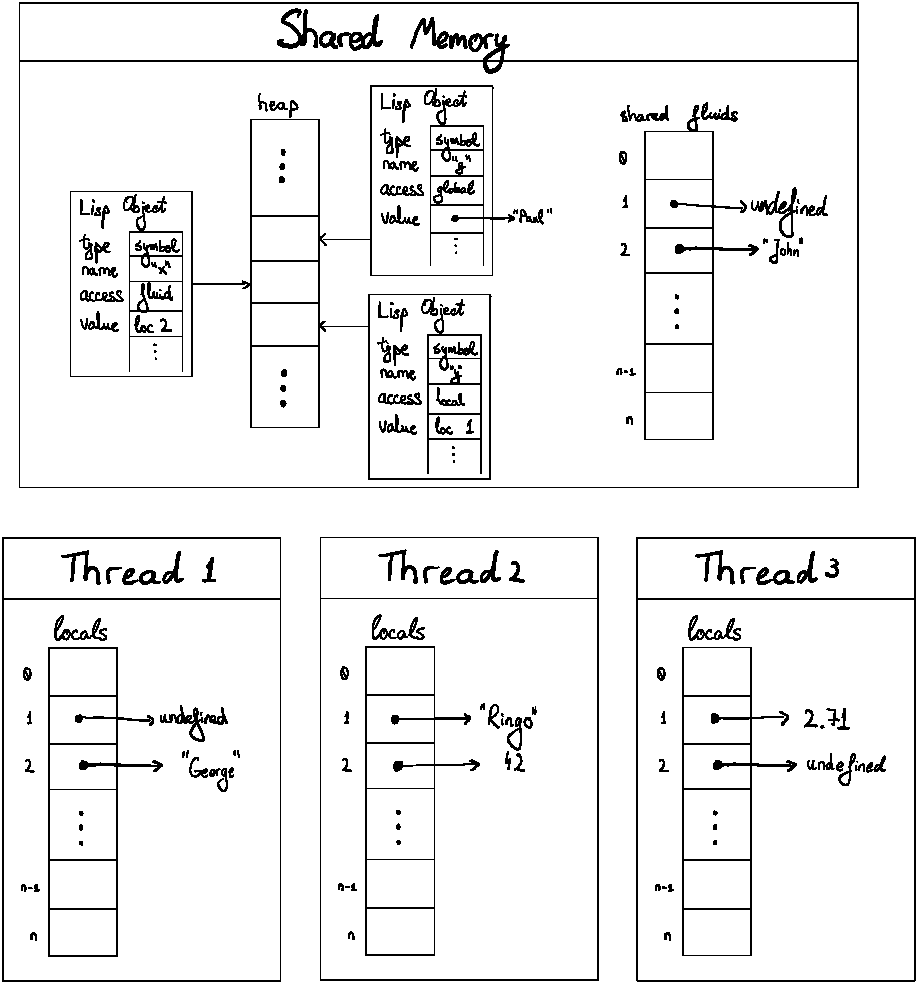
\includegraphics[width=0.9\linewidth]{symbols.pdf}
  \caption{Storage of symbols in ParVSL}
  \label{fig:symbols}
\end{figure}

In figure \ref{fig:symbols} I show a full example of how symbols are stored. The first symbol is \texttt{g}, which
is a \emph{global} symbol. It's value is stored directly in the global heap (like in the original VSL). The symbol \texttt{x}
is \emph{fluid}. It's heap value simply indicates a location (\texttt{loc 2}). We use the index to find the actual value
in thread-local storage. Threads 1 stores the string \texttt{"George"} while thread 2 stores the integer \texttt{42}.
Thread 3 has not bound any local value to the symbol so it is \texttt{undefined}. However, it can still access the
global value in \verb|shared_fluids|, the string \verb|"John"|. Finally, symbol \verb|y| is \emph{local}. It is
undefined in \verb|shared_fluids| but otherwise behaves the same as \verb|x|, storing its thread-local values at
index \verb|1|.

I redesigned shallow binding to use a RAII style class, called \verb|Shallow_bind| which deals with all the changes
described above, while providing more safety guarantees, thus leading to more robust code. It checks if the symbol is global and prevents binding,
it handles thread-local storage and it always restores the old value correctly in its destructor, including the
case of exceptions. Previous code spent time testing error flags, manually restoring the old value in every place.
For example, the code in \ref{code:let-vsl} was rewritten as:
\begin{code}
\begin{verbatim}
void implement_let(string varName, LispObject expr1, LispObject expr2) {
  LispObject symbol = lookup_symbol(varName);
  Shallow_bind bind_var{symbol, eval(expr1)};
  eval(expr2); // evaluate the rest of the code
}
\end{verbatim}
  \caption{Implementation of \texttt{let} in ParVSL.}
  \label{code:let-parvsl}
\end{code}

\section{Data races in the interpreter}
\label{sec:datarace}

Running VSL in parallel involves, in effect, running an interpreter in each thread. The spawned threads do not
run a read-eval-print loop, instead they run a computation, save the result, then terminate. However,
in ParVSL I allow these threads to execute any code the main thread can, with no restriction. This means
all threads can use and modify global state and interact with standard input, output and files and
thus can conflict with each other.

There are plenty of global variables holding state in VSL. I discovered which ones represented local
state.
One example is \verb|unwind_flag|, which is heavily used for Lisp control flow. Among other uses, it is
mutated to indicate an exception, to implement \verb|goto| and \verb|return| instructions,
as well as to indicate early program exit,
among other uses. Each thread needs its own version of this global flag, otherwise they will mess with each
other's control flow, so I made it \emph{thread-local}.

A third case is file handling. Global variables indicate which file is in use, and hold buffers for reading
and writing. Again, I had to make all these thread-local. On the other hand, there are other variables holding
truly global information, like file handles. At one point I was over-zealous in
my modifications and made a variable thread-local which should have stayed global. Although tt looked as if it indicated
the direction of the current file, it turned out to be a bitmap of all the files in the system. The fact
that VSL makes creative uses of integers for optimisation reasons effectively hides information from the type system.
After a significant time spent debugging, I realised that the variable was used differently and the solution became apparent.
I also modified the variable to use a proper \emph{bitset} data structure, enhancing readability.
As a bonus, ParVSL can now support a much larger number of open files than the 32 imposed by the size of integers.

Those globals which are not thread-local still pose the problem of data races. For instance, multiple threads
may try to read from or write to the same file. ParVSL cannot avoid contention altogether: those conflicting
operations will be serialised non-deterministically. However, it is important to prevent these data races at
the C++ level, because they cause undefined behaviour, ultimately leading to anything from spurious crashes
to more subtle data corruption.

I changed all functions for opening, closing, or altering a file to use mutex locks, with one mutex per file.
Opening and closing files are not on the critical path of the interpreter so time was less of a concern.
However, reading and writing can be part of the main loop. Many programs will run from a file, not standard input,
and it is common to print regularly to standard output or file. To manage this, I added extra per-thread buffers
to handle single character reads and writes. Then, I only synchronise threads when flushing the buffers, reducing
contention. In my testing, these changes did not slow down ParVSL in any measurable way.

\section{Threads and synchronisation in ParVSL}
\label{sec:threads}

At the start of the project I bolted on to ParVSL a small, broken, but very much useful feature to evaluate
Lisp code in a new thread, as demonstrated in section \ref{sec:babythreads}. I ran a number of small tests
and found where this functionality broke the interpreter, then reworked those parts of the Lisp system
until it successfully passed the tests. At the same time, I adapted a large suite of regression tests
from REDUCE to ensure single-threaded behaviour was unaffected and performance didn't degrade significantly.
Once I was confident that ParVSL could run multi-threaded I started implementing the extra functionality
required to make parallel programs practical.

To start a thread, the user needs to call the \verb|thread| function.
Originally, the function only took a Lisp expression as argument and evaluated it. This was highly impractical,
as the expression was passed unevaluated and data could not be passed naturally. The only way to allow
communication was to write the data into a global symbol and have the code executed access that symbol.

I changed the implementation of \verb|thread| to instead accept a function function name and the argument list
as arguments. The arguments can be local symbols, and their values will be correctly bound to parameter names
within the thread. The spawned thread then applies the function to the arguments and saves the result
before terminating. The return value of \verb|thread| is the thread id, which then has to be used to
join the thread. Calling  \verb|join_thread| on the thread id, will block until the thread has finished
executing, and retrieve the resulting value of the computation.

\begin{verbatim}
tid := thread('add, {2, 3});
result := thread_join tid;
print result;
> 5
\end{verbatim}

My implementation minimises overhead. The list of arguments is managed on the heap which is visible by all
threads, so a simple pointer is enough to pass them. Furthermore, all unjoined threads and corresponding return values
need to be tracked.
A hashmap from thread ids to return values is updated when thread execution is completed.
Consequently, when \verb|thread_join| is called this value is returned and removed from the hashmap. All threads
have unique ids for the lifetime of the program, so there are never any conflicts in the hashtable.
Starting and joining a thread are synchronised under a mutex lock to prevent data races.

I was careful to prevent the garbage collector from collecting these parameters and return values.
Starting a thread is GC-safe: garbage collection will not initiate while a new thread is starting up. This ensures
that threads are always in a safe state and registered in the thread-table correctly during garbage collection.
At that point, function parameters are tracked just like regular variables so they will be safe from GC.
However, return values are stored past the lifetime of their respective threads, so I add them
to the unambiguous root set at the beginning of garbage collection.

\subsection{Mutual exclusion and condition variables}

It is not enough for the user to be able to spawn threads. ParVSL has a shared memory model so at a minimum
it has to provide a way to mechanism for mutual exclusion. I exposed the C++ \emph{mutex locks}
with a very simple interface:

\begin{verbatim}
m := mutex();
mutex_lock(m);
mutex_unlock(m);
\end{verbatim}

The mutexes are created in C++ and stored in a lock-free hashtable, each with a unique id. I used the lock-free
hashtable implementation to allow different mutexes to be accessed in parallel. I also
make use of the \verb|Gc_guard| when \verb|mutex_lock| is called. This is to ensure that the blocking
call to lock the mutex does not cause a deadlock during garbage collection.

While ParVSL users can use mutexes to protect against data races, they may not always do so
(due to omissions or bugs). Operations such as modifying a global symbol or mutating a list in place
may still clash.
One way to ensure safety would be to lock the mutex for any such operations, but this change would add a
too much overhead to ParVSL. With this in mind, the decision was made to leave this issue as a responsibility
of the ParVSL user, since they can manage the trade-off between safety and lock usage minimisation.

The second primitive that I added was \emph{condition variables}. They provide a useful way for
threads to signal each other, enabling an efficient way to perform common parallel processes such as
waiting for a task to finish. I stored the condition variables the same way as the mutexes (i.e. in a lock-free
hashtable) and the wait operation uses the \verb|Gc_guard| to check for garbage collection.

I included a few more helpful function such as \verb|hardware_threads| to check the number of hardware
threads on the current system, \verb|yield| to allow the system to reschedule the thread, and
\verb|sleep| to pause the thread for a specified duration.

These primitives are versatile enough to enable parallel algorithms, as I will showcase in Chapter \ref{ch:evaluation}.
They can also be used to implement other common threading gadgets, such as atomics and futures
(see \ref{ssec:managethreads} and \ref{ssec:waitjob}).

\section{Saving state to disk and reloading}
\label{sec:preserve}

REDUCE has an important feature which allows the user to preserve the state to disk. A \texttt{preserve} instruction can be
used to do so, and the user is able to specify a function to run on restart. \verb|preserve| saves the entire state of the
program, including memory and symbols.

It is difficult to keep the same guarantees when multiple threads are running.
If a thread attempts to preserve while others
are running, the contents of the final image will be non-deterministic and generally undesirable,
even if all data races were resolved. At the same time, I found little benefit to implementing such
a feature, as the ability to preserve is useful in retaining the results of computations, not intermediate states.
Saving state to disk is used at the end of the program.

Once all threads are joined and there is only one thread running, all the
thread-local data can be treated as global again and stored in the same locations that
VSL uses. When restoring from an image, this data is moved back into thread-local storage. The image
format is not affected.


\chapter{Evaluation}
To evaluate the project, I worked with existing REDUCE code for regression testing
but also wrote my own tests in both plain Lisp and RLISP code.
Bracketed Lisp code was useful at the beginning of my project when ParVSL was not
fully functional and I needed unit tests, while RLISP was necessary to write
more complicated code which interfaces with REDUCE.

\section{Single-threaded building of REDUCE}

My project involved modifying a large body of code and it was almost guaranteed
that I would introduce bugs during development. Thankfully, the language and its
direct application are well intertwined, so there is a very large coverage test already
available to demonstrate most functionalities of the language: building REDUCE.

REDUCE consists of around 400 thousand lines of code, and since VSL was built to
run it, all functionality in VSL is being used in REDUCE. In addition to that,
REDUCE comes with a comprehensive suite of regression tests for most packages.
These tests involve a large amount of heavy computation, stress testing
many different algorithms, using large amounts of memory and requiring multiple cycles
of garbage collection.

Between building REDUCE and passing its tests, I can detect development bugs and be
confident that ParVSL retains backwards compatibility. Any error while running the code,
or any difference in output between VSL is considered a bug. This approach helped me
find most of the bugs in my code. The disadvantage was that when I had to debug there
was too much code running and it was difficult to pinpoint the source of the problem.

To aid with this, I had multiple stages to build. The first stage was just building
the core, while the second involved building the libraries. If an error showed up while
building a library, most other libraries could be skipped to help pinpoint the problem.

\subsection{Bugs in VSL and REDUCE}

While debugging I discovered some issues in VSL. The language hadn't been tested
extensively until I started working on it. These issues were mostly minor. Some functions
were not present at all and needed to be reintroduced, for example a system function to get
the working directory. There were subtle bugs such as wrong
hard-coded strings and integers. There were multiple issues with floating point manipulation,
again caused by simple human errors (e.g. negated condition being checked). Switching between
output files would lose buffer content. In one place, a value on the heap was not marked
properly, meaning that if a garbage collection was triggered at the right time, it would
be collected prematurely, causing corruption. All these bugs have since been fixed
in both VSL and ParVSL.

REDUCE itself showed multiple cases of sloppy code. Most of the time, the issue was using
a global symbol with a very common name liberally and then behaving weirdly
on clashes. The most striking example was when the RLisp interpreter used the symbol \texttt{x}
during parsing, meaning any tests using the variable \texttt{x} as a free global value
would turn it into a self-reference to code.
Another instance was a name clash in the error handling function, leading to failure
to contain exceptions. While these cases have been fixed, there are many other
such potential problems within the REDUCE packages which will have to be cleaned up.
% Identifying when odd behaviour was down to my code or whether it revealed

\subsection{Benchmarks}

In addition to helping me find issues in ParVSL, building REDUCE also provided a
good performance benchmark. The building process simply runs Lisp and RLisp code so
running it in VSL and ParVSL will showcase the performance difference between the
two in a single-threaded case.

Figure \ref{fig:single-threaded} shows the relative performance of ParVSL compared to VSL.
RCORE is the core of REDUCE, skipping non-essential packages from the build. ALG TEST is
a set of regression tests normally used to check for bugs in the code. INT TEST tests the
symbolic integration package, and provides a good performance benchmark.

\begin{figure}[H]
  \centering
  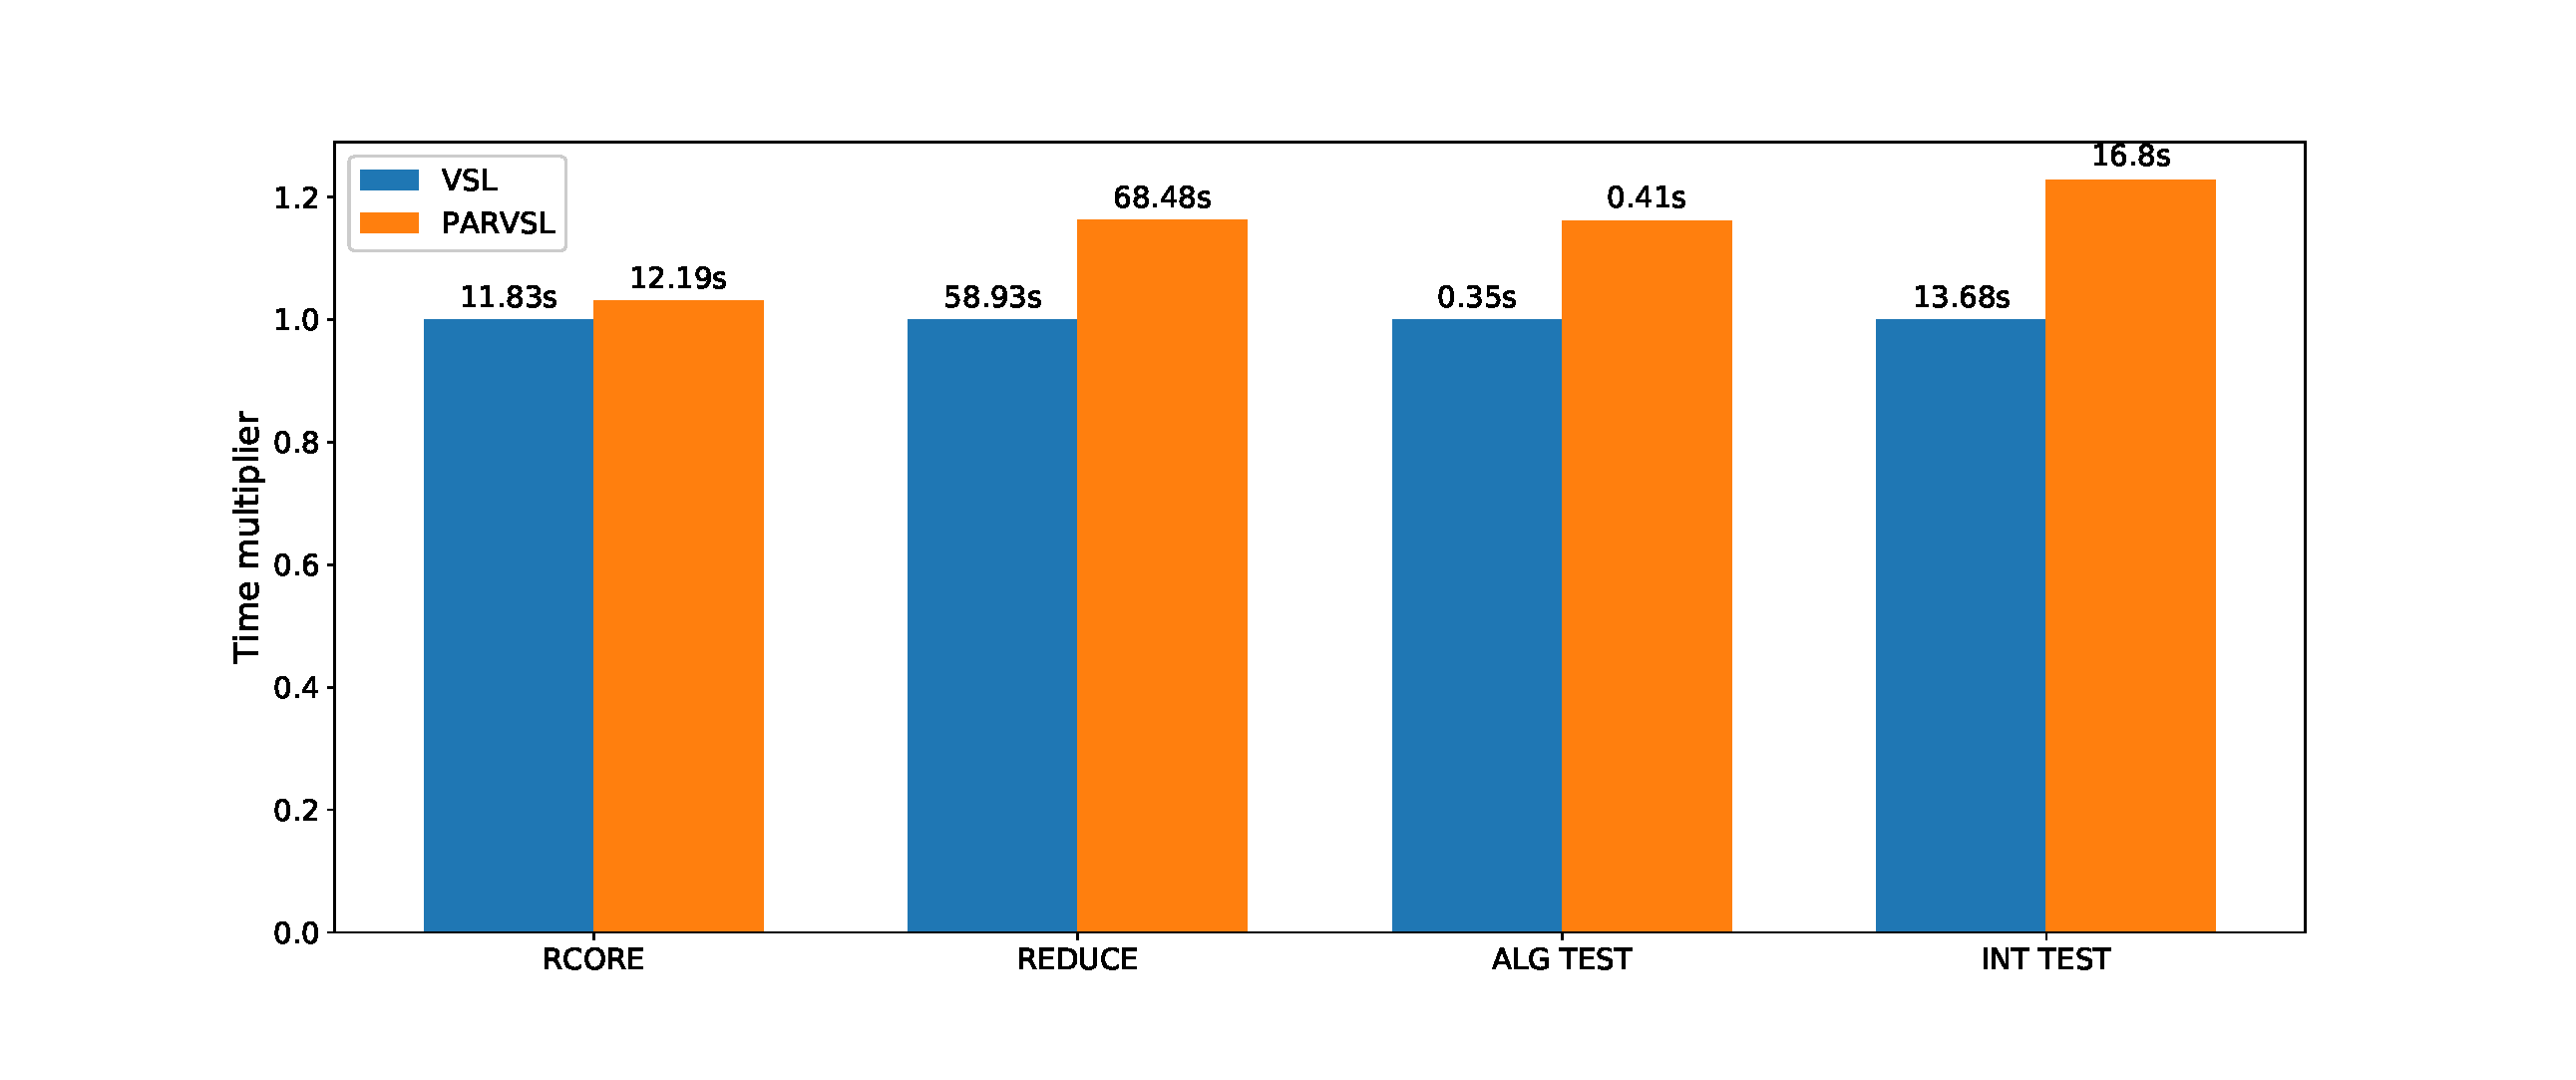
\includegraphics[width=1\linewidth]{single_threaded.eps}
  \caption{Relative performance of ParVSL on single-threaded tests (lower is better).}
  \label{fig:single-threaded}
\end{figure}

A slow-down between 5 and 20 percent can be observed. I have used the GProf \cite{gprof}
tool to profile the code and found the biggest cause of the time difference is the
symbol value extraction mechanism described in \ref{sec:symbols}. In VSL all symbol
values are stored globally with the symbol, whereas ParVSL adds extra book-keeping.
The symbol access function is on the critical path, and slows the code by at least
five percent. I have also compiled a version of ParVSL with the new symbol
storage disabled. In the above tests, it is less than 5\% slower than VSL, showing
that this is the biggest factor, even though in theory it is an $O(1)$ operation.
This penalty would easily be eliminated in a compiled language, where the
checks for global and fluid variables could be performed statically and optimised away
from the runtime.

\section{Multi-threading unit tests}

While REDUCE provides a large suite of tests for single-threaded behaviour, I had to come
up with new tests for multi-threading. Before going into larger examples, I started with a small
suite of unit tests in Lisp.

The following test shows multiple threads sharing a variable. They have to acquire
a mutex to prevent a data race. All they do is increment it by one, so the final
value should be equal to the number of calls.

\label{lst:shared-global}
\begin{verbatim}
(global '(x x_mutex))
(setq x 0)
(setq x_mutex (mutex))

(de incr_x ()
  (mutex_lock x_mutex)
  (setq x (add1 x))
  (mutex_unlock x_mutex))

(dotimes (i 10000) (thread '(incr_x)))
(print x)
> 10000
\end{verbatim}

When modifying the garbage collector, I had issues when multiple
threads were initiating it, for example I discovered a deadlock
with my original GC locks (section \ref{sec:gclock}), which I then
quickly fixed. It was easily reproduced with the following test:

\begin{verbatim}
% reclaim forces garbage collection
(dotimes (i 16) (thread '(reclaim)))
\end{verbatim}

Big numbers use continuous areas of memory and can easily
fill in entire segments all at once. The code below simply
raises numbers to a large power in parallel. It helped me discover
that my code was not handling an allocation request being
larger than the segment size.


\begin{verbatim}
% a naive recursive power function
(de pow (a b)
  (cond
    ((zerop b) 1)                  % if b = 0: return 1
    (t (times a (pow a (sub1 b)))) % else: return a * pow(a, b - 1)
  ))

(dotimes (i 1000)
  % raise i^i for really large numbers
  (thread 'pow (list i i)))
\end{verbatim}

These tests, among others, were very helpful in finding bugs
during development. They were added when testing new functionality,
sometimes as a result of finding a bug in a larger example.
They now act as regression tests for ParVSL.

\section{Thread pool}

Once I showed  that ParVSL could run both single-threaded code (i.e. build REDUCE) and pass some
simple tests for multi-threading, I was able to write more complex code using threads.

Spawning hardware threads directly to parallelise each task can be undesirable. The user has
to manage the lifecycle of each thread, making sure to join it and also to manage the number
of available threads on the current hardware directly. Failure to do so will quickly result in
over-subscription of threads. Each thread object comes with its own overhead including a local
stack and operating system handle,

A thread pool is a structure for simplifying parallelism by abstracting away the interaction
with hardware threads. A thread pool consists of a work queue for pending jobs and a number
of worker threads which execute those jobs as they become available. The number of workers
can be kept low so that the program never has to spawn more threads
than the operating system limit, and threads can be reused. Once a thread pool is created,
the user simply needs to submit jobs and they will be automatically parallelised.

\subsection{A thread-safe queue}

The main data structure behind the thread-pool is a thread-safe queue. All threads may push
jobs to this queue and all working threads pop tasks from it to execute. Jobs can be executed
in any order, but I used a FIFO queue so that they would be executed in the order they are submitted,
which seemed the most natural.

We can implement such a queue easily in ParVSL using a mutex and a condition variable.
I wrote the following code in RLisp, since the thread pool will be useful in parallelising
REDUCE code.
We start from a simple queue, with the following functions:

\begin{itemize}
\item \texttt{queue()} creates a new queue
\item \texttt{queue\_push(q, x)} pushes value \texttt{x} to queue \texttt{q}
\item \texttt{queue\_pop(q)} pops and returns the value at the front of the queue
\item \texttt{queue\_empty(q)} checks if the queue is empty
\end{itemize}

A thread-safe queue is simply a wrapper on top of the normal queue:
\begin{verbatim}
procedure safe_queue();
  {queue(), mutex(), condvar()};
\end{verbatim}

We need two procedures: \verb|safe_queue_push(sq, x)| and \verb|safe_queue_pop(sq)|. The latter will
wait if the queue is empty until an element is enqueued. The waiting is done using the condition variable:

\begin{verbatim}
procedure safe_queue_pop(sq{q, m, cv});
begin
  mutex_lock m;

  while queue_empty q do
    % wait for another thread to push an element and notify
    condvar_wait(cv, m);

  res := queue_pop q;
  mutex_unlock m;
  return res;
end;
\end{verbatim}

Now, the push method must notify the condition variable if the queue was empty.
\begin{verbatim}
procedure safe_queue_push(sq{q, m, cv}, x);
begin
  mutex_lock m;
  queue_push(q, x);
  condvar_notify_one cv;
  mutex_unlock m;
end;
\end{verbatim}


\subsection{Managing threads}
\label{ssec:managethreads}

With the queue implemented we can design the worker threads. The starting thread
initialises the queue and starts all the workers as individual threads. It can start
either the maximum number of hardware threads (which can be determined using the
\texttt{hardware\_threads()} function), or a custom count. Each thread is passed a reference to
the thread pool, so it can access the queue. Once the threads are started, they will only
be joined on exit or when the user manually stops the pool.

The mechanism for stopping the queue is a simple atomic flag. Atomics are not offered as
a primitive in ParVSL, but can be easily implemented with a mutex lock. There is no direct
mechanism for interrupting a thread running a task\footnote{C++ does not provide this as a
primitive and indeed if a thread was interrupted in the middle of a system call or while
holding a mutex lock it would cause all sorts of problems.}, but workers can check the flag
every time before taking a new task from the queue.

When the the user tries to stop an empty pool, all
the workers will be in a sleeping state, waiting for the queue condition variable to be
notified and causing a deadlock.

\begin{verbatim}
while atomic_get(run_flag) = 'run do
  // The workers can get stuck here waiting on an empty queue
  job := safe_queue_pop(sq)
  run_job job;
\end{verbatim}

Another idea is to not use a blocking call to pop from the queue, but rather spin:
\begin{verbatim}
while atomic_get(run_flag) = 'run do
  job := safe_queue_try_pop(sq)
  if job then
    // trypop succeeded
    run_job job
  else
    // important to yield here
    thread_yield()
\end{verbatim}

This approach solves the issue, but it is important to note the \verb|thread_yield()| call,
which I implemented to directly call the C++ equivalent. It allows the
system to schedule other threads to do more work, preventing starvation.

\subsection{Waiting for a job's result}
\label{ssec:waitjob}

In ParVSL, the \texttt{thread} function takes another function to execute on the new thread,
along with the arguments for that function. The return value of the function call is
then recovered when joining the thread with \verb|join_thread|, enabling thread communication.

When switching from threads to jobs in the thread pool, we want to maintain this functionality,
otherwise the only way to communicate between parallel jobs would be through global state,
which would severely limit its usefulness. Passing arguments for a job is trivial, as they are simply
stored in the safe queue, along with the function to be called. However, returning the result of
a job required extra book-keeping.

Using the primitives in ParVSL, we can implement a \texttt{future} type. A future is a mechanism
that allows us to both wait for a task and obtain its return value. A future starts out as empty.
It can have any number of readers but only one writer. The writer is usually the creator of the future
and will set its value exactly once, at some point after creation. The readers can then try to get the
value inside the future. If the future is fulfilled, the get call returns instantly. Otherwise, it
becomes a blocking call, waiting until the future is set, then returning the respective value.

Implementing a future is similar to the safe queue, using a mutex and a condition variable.
Getting and setting the future requires acquiring the lock. The getter has to wait on the condition
variable if the future is not set. The setter notifies all the getters after setting the value.
The full implementation can be found in Appendix \ref{sec:threadpool-code}.

With the future implemented, we can finish the thread pool, having a mechanism for pushing a job:

\begin{verbatim}
procedure thread_pool_add_job(tp, fn, args):
  fut := future()
  safe_queue_push(tp.safe_queue, {fn, args, fut})
  return fut
\end{verbatim}

The caller can use the future to wait for the result of the job and the workers need to set the future
when finishing a job. Finally, I note that the thread pool must deal with exception handling. The worker threads
need to catch any error while running the job and report it through the future. Initially, I failed to include
it meaning that worker threads unwound unsafely. This lead to the the thread-pool being unable to signal the
thread and fail to terminate. Additionally, threads waiting for the result would also be stuck.

There are many aspects to be considered in the design of a thread pool. I have focused on the main ones, and
this thread pool was sufficient for the rest of evaluation. I have successfully used it to parallelise the
other experiments in this report. However, depending on the task it could be improved upon with more features.
Currently, the number of threads is static, but it could dynamically start and stop threads to accommodate
the workload. An efficient safe queue could be implemented using more granular locking. Furthermore, we could
reduce contention on the queue by having each worker keep its own queue, and the main queue would act as a
dispatcher.

\section{Implementing Parallel Mergesort}

To test the correctness and performance of ParVSL I implemented a few classic algorithms that are relatively
easy to parallelise. Sorting is a particularly good example. Mergesort splits a list in two, sorts each half
recursively, then merges the results to obtain the sorted list. Sorting the individual halves can be done
in parallel.

\begin{verbatim}
tp := thread_pool()

procedure parallel_merge_sort(list):
  if length(list) < 2:
    return list

  xs, ys := split(list)
  sorted_xs_future := thread_pool_add_job(tp, 'parallel_merge_sort, {xs})
  sorted_ys := parallel_merge_sort(ys)
  sorted_xs := future_get(sorted_xs_future)

  return merge(sorted_xs, sorted_ys)
\end{verbatim}

We can use the thread pool implemented above to achieve parallelism. Without the thread pool, we would
have to manually manage threads. Using threads here would have resulted in a new thread spawned for
each element in the list. The function would already oversubscribe threads for lists as small as
100 elements. The thread pool only uses a constant number of threads.

\subsection{Dealing with tasks waiting for other tasks}

However, the naive implementation above is incorrect and it will deadlock as soon as the number of
jobs exceeds the number of workers. This highlights a shortcoming of the thread pool. In its current
state is does not handle tasks enqueuing and then waiting for other tasks. In this case, all the workers
will end up waiting for the future (\verb|sorted_xs_future|) without doing any work.

To fix this, I have added extra functionality to the thread pool. An extra procedure \verb|thread_pool_run_job|
can be called by any thread to run one job from the queue. This procedure is implemented similarly
to the worker function, except it takes at most one job (or none if the queue is empty) from the
queue instead of looping.
This function should be called by any job which is waiting for another job in the thread pool.

I also needed to implement another function for futures \verb|future_try_get|, which only returns the
value in the future if it was fulfilled, without blocking, or indicates failure, without blocking.

Subsequently, I have changed line the \verb|future_get| call above to the following code:
\begin{verbatim}
while null(future_try_get(sorted_xs_future)) do
  thread_pool_run_job(tp);
\end{verbatim}
Now, workers can start (and finish) other jobs while waiting and will not deadlock.

\subsection{Results}

To test the correctness, I simply generate a list of random numbers, then compare the output
to that of the sorting function built in REDUCE. Afterwards, I could test for performance.
I first tuned the parallel version to use the sequential algorithm once if the list is too
small. I found on my machine that around parallelisation became useful once the size of
the list was larger than 1000. Without this optimisation
the parallel version would spawn too many jobs (as many as \(O(N)\)) and the time spent book-keeping
would completely eliminate any benefit of multi-threading.
Table \ref{table:parmergesort} shows the performance improvement
we can gain by increasing the worker count on a computer with 4 physical CPU cores.

\begin{table}[H]
\centering
\begin{tabular}{rrrrr}
& \multicolumn{4}{c}{Number of workers} \\
List size & & & \\
($\times$ 1000) & 1 & 2 & 8 & 16\\
\hline
100  & 2.351 & 1.563 & 1.319 & 1.071 \\
250  & 5.282 & 3.409 & 2.554 & 2.137 \\
500  & 11.152 &  5.850 & 4.906 & 3.995 \\
1000 & 22.840 & 11.706 & 9.054 & 7.514 \\
\end{tabular}
\caption{Parallel merge sort times by number of workers.}
\label{table:parmergesort}
\end{table}

\section{Multiplying polynomials in parallel}

Polynomials are widely used in computer algebra. Being able
to multiply two polynomials is a fundamental problem in computer
algebra with for a plethora of applications ranging from
including symbolic integration and computational geometry,
so speeding it up with multi-threading could prove to be quite valuable.

At the same time, it is relatively easy to split the multiplication
algorithm into multiple independent tasks. All the well-known
multiplication algorithms (i.e. the naive quadratic solution, Karatsuba,
and using the Fast Fourier Transform) have parallel versions \cite[Chapter~30.3]{cormen}.
The latter are mostly used for multiplying numbers, and REDUCE
uses the quadratic algorithm as it is better suited to sparse and
more general multi-variate polynomials.

I wrote a parallel implementation of polynomial multiplication in REDUCE
and ran it in ParVSL. It splits the polynomials into odd and even
terms and thereby splits the problem into four sub-tasks (multiply every combination).
These can be easily computed in separate threads, then joined to obtain the
resulting polynomial. While the small test case only covers uni-variate
polynomials the results I show might reasonably be expected to apply to
more general cases.

% \begin{table}[H]
%   \centering
%   \begin{tabular}{rrrrr}
%   Poly size & VSL & ParVSL \\
%   \hline
%   1000 & 0.660 & 0.480 \\
%   2000 & 1.588 & 0.941 \\
%   3000 & 3.280 & 1.729 \\
%   4000 & 5.486 & 2.834 \\
%   5000 & 8.182 & 4.177 \\
%   \end{tabular}
%   \caption{Parallel multiplication of polynomials vs single-threaded.}
%   \label{tab:parpolymult}
% \end{table}

\begin{figure}[H]
  \centering
  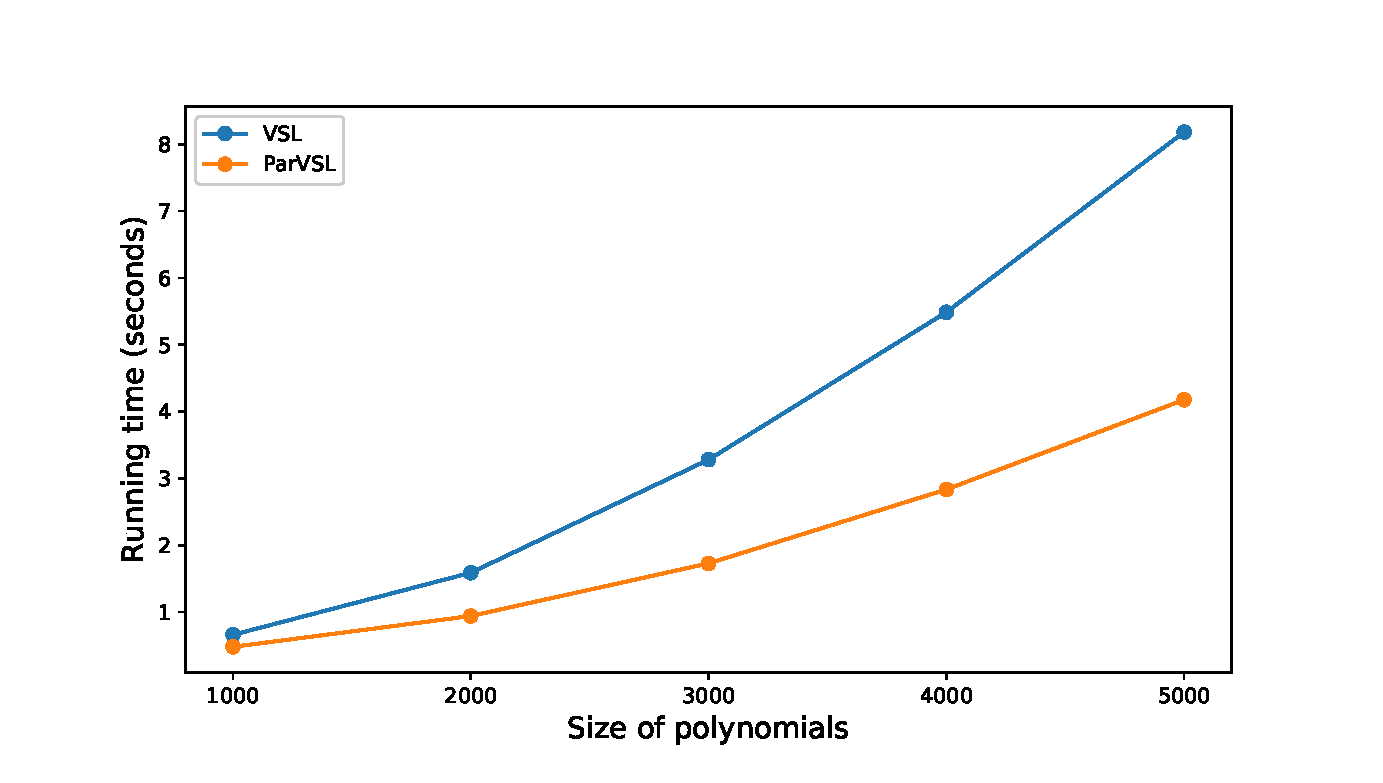
\includegraphics[width=0.8\linewidth]{polymult.eps}
  \caption{Running time of polynomial multiplication in parallel vs single-threaded (lower is better).}
  \label{fig:parpolymult}
\end{figure}

% For small polynomials just gaving the thread infrastructure may
% tend to hurt. After all if you take two quadratics and split them
% into bits to try to multipoly in parallel you are liable to lose!
% For big enough polynomials there can be a saving reasonably consistent
% with the number of threads your CPU can support, and one can then
% suggest that for heavy algebra users that could really help.
% [obviously] if one increases the thread count beyoind the level your
% CPU provides there is no benefit, and possibly ahead of that memory
% bandwidth starts to get saturated, so one does not really expect a
% full factor of 8 on an 8-core machine!
% Your test code does just univariate polys but the results you show
% might reasonably be expected to apply to more general cases, and
% polynomial multiplication is such a fundamental operation in algebra
% that being able to speed it up could really help.

\section{Gröbner basis}
\label{sec:groebner}
\emph{Gröbner basis} \cite{Groebner} is a set of non-linear multivariate
polynomials that has useful algorithmic properties for many important problems
in mathematics and sciences, including computational geometry, linear programming
and coding theory. Here, a basis is just a set of polynomials. A basis is a Gröbner basis if
all leading power products of linear combinations of polynomials in the basis
are multiples of at least one of the leading power products in the set.

The problem of constructing Gröbner bases for polynomials is characterised as follows:
given a finite set of multi-variate polynomials $F$ in $K[x_1,\dots,x_n]$, find a
finite set of polynomials $G$ in $K[x_1,\dots,x_n]$ such that $ideal(F) = ideal(G)$
and $G$ is a Gröbner base.
Any set of polynomials has a Gröbner basis, which is an equivalent system.
In the case of linear systems the problem specialises to Gaussian elimination,
while in the case of systems of univariate polynomials, it specialises
to Euclid's algorithm. As such, it is a generalisation of the two, further
covering non-linear systems in multiple variables. Problems which are extremely
difficult to solve for arbitrary bases (such as solving a non-linear system of equations)
may be solved easily for their equivalent Gröbner basis.

Buchberger's algorithm \cite{Buchberger} is used to find the Gröbner basis
of a set of polynomials. It involves repeatedly applying special reductions
on pairs of polynomials to update the current base until it converges.
A mathematical definition of Gröbner bases, along with an explanation of
the algorithm can be found in Appendix \ref{ch:grobner}.

\vspace*{.2cm}
\begin{code}
\begin{algorithm}[H]
  \SetKwInOut{Input}{Input}
  \SetKwInOut{Output}{Output}
  \SetKwData{B}{$B$}
  \SetKwData{G}{$G$}
  \SetKwData{F}{$F$}
  \SetKwFunction{Spoly}{S-polynomial}
  \SetKwFunction{Reduce}{Reduce-by}
  \Input{A basis $F$}
  \Output{A Gröbner basis $G$ such that $ideal(F) = ideal(G)$.}
  $\G \leftarrow \F$\;
  \B $\leftarrow \{(p_1, p_2) \mid p_1,p_2 \in G \land p_1 \neq p_2 \}$\;
  \While{\B $\neq \emptyset$} {
      $(p_1, p_2) \leftarrow$ an element of \B\;
      $B \leftarrow B \setminus \{(p_1, p_2)\}$\;
      \tcp{See Appendix \ref{ch:grobner} for a description of these functions.}
      $s \leftarrow$ \Spoly{$p_1$,$p_2$}\;
      $s \leftarrow$ \Reduce{$s$, $G$}\;
      \If{$s \neq 0$}{
        $B \leftarrow B \cup \{(s, p) \mid p \in G\}$\;
        $G \leftarrow G \cup \{s\}$\;
      }
  }
  \caption{Buchberger's algorithm for finding the Gröbner basis of a set of multi-variate polynomials.}
\end{algorithm}
\label{alg:buchberger}
\end{code}
\vspace*{.2cm}

REDUCE offers a \verb|Groebner| package for computing Gröbner basis which I tried
to improve using parallelism. The known upper bound on the degrees of elements
in the computed basis is $O(d^{2^n})$, where $n$ is the number of variables
and $d$ is the maximum total degree of the polynomials \cite{MAYR}. This means the
algorithm can have super-exponential runtime, and its performance highly
depends on the order in which it applies the reductions.

I implemented a parallel version of the algorithm which uses a work
pool to try reductions in parallel, maximising the chance of finding the most useful reductions
faster.

The most challenging problem was finding good tests for my algorithm.
Most examples I found were either trivial and were computed in under one
second, or never terminated after hours of runtime. Coming up with
tests that do not fall in either category requires an advanced understanding
of the maths behind non-linear systems. My supervisor helped me
find an input which terminates in under a minute, than modified it
to contain a large number of dependent equations to increase the complexity.

Figure \ref{fig:groebner} shows the results. Each test was run three times
a six-core CPU and computer, explaining the levelling in runtimes after
six threads. The variance was under 3 seconds in this case so I omitted it.

\begin{figure}[H]
  \centering
  \includegraphics[width=1\linewidth]{groebner.eps}
  \caption{Running time of Buchberger's algorithm by number of threads (lower is better).}
  \label{fig:groebner}
\end{figure}

I also found another interesting test in which the parallel version
always succeeded in under 2 seconds, whereas the single-threaded algorithm
crashed VSL. I determined that the parallel algorithm added inherent
non-determinism which effectively shuffled the reductions and
reduced the probability of getting stuck.
To compensate for this in VSL, I added a shuffling stage in both algorithms
when updating the set of pairs $B$. This change did not affect the parallel
algorithm, but it did make the sequential algorithm terminate sometimes.
I then ran both algorithms 1000 times on the same test. The parallel
algorithm always succeeded in finding a Gröbner basis in seconds,
while the sequential algorithm timed out after one minute in 116/1000 runs.
Therefore, the parallel Buchberger implementation is not only faster,
but also more robust, as the level of concurrency it affords significantly
reduces the chance of encountering a pathological case.

\section{Parallel building of REDUCE}

Most of REDUCE is made up of RLISP code, which can be run in VSL or ParVSL
to generate a build. The process can be separated into two steps:
building the core of REDUCE, and then building all the additional packages.
The core, which I will refer to as RCORE, satisfies most of the dependencies
any of the additional packages need, and only takes a fraction of the time
to build.

\begin{table}[H]
\centering
\begin{tabular}{lr}
 & Time (s)\\
\hline
RCORE & 11.83s\\
REDUCE & 59:93s\\
\end{tabular}
\end{table}

A good use of multi-threading would be to speed up this build time by
arranging to build individual REDUCE packages in parallel. The RCORE base
should still be built sequentially, as it is much more difficult to
separate it into independent tasks. However, the rest of the packages mostly
only have RCORE as a dependency.

I extracted a list of 64 packages to build. The starting point was the
RCORE image. On VSL, I simply ran the building sequentially:

\begin{verbatim}
for package_name in packages do
  build_package package_name;
\end{verbatim}

The total running time was 14.1 seconds. Then, I used the thread pool
to run these builds in parallel:

\begin{verbatim}
tp := thread_pool(hardware_threads());

pack_futures := {};
for package_name in packages do <<
  pack_future := thread_pool_add_job 'build_package {package_name};
  pack_futures := pack_future . pack_futures;
>>;

% We need to ensure all jobs are finished.
for pack_future in pack_futures do
  if (future_get pack_future) != nil do
    print "error building package";
\end{verbatim}

Running this code will initially fail building any package. This is caused
by global side-effects of building the packages. The first issue is that all
packages use global symbols with common names for storage. Any global
symbol used by a package should use a globally unique name, usually by prepending
the package name to the symbol name. Unfortunately, the writers of these packages
didn't always follow good practices. It is outside the scope of this project to
fix all REDUCE packages, however I tried to work my way around that.

I modified the ParVSL code so that when I enable a compilation flag it tracks all
reads and writes to global values of fluid or global symbols. Afterwards, I wrote a Python
script which builds each package individually with the build flag on and saved those
accessed to a file. The script computed all conflicts between packages,
then generated a REDUCE test file which would remove all global access on building the packages:

\begin{verbatim}
% Force conflicting symbols to be fluid.
% Here, global1, global2, etc. are the names of those conflicting symbols
fluid '(global1 global2 ...)
fluid '(store!-global1 store!-global2 ...)

store!-global1 := global1;
store!-global2 := global2;
...

procedure build_package_safe(name);
begin
  % we bind the conflicting variables locally
  scalar global1, global2 ...;

  % restore their original global values inside the local scope
  global1 := store!-global1;
  global2 := store!-global2;
  ...

  build_package(name);
end;
\end{verbatim}

The generated file makes use of the dynamic scoping mechanism in Lisp. When building the package
with \texttt{build\_package\_safe}, all accesses to those global symbols will instead access locally
bound ones. This removes all conflicts between symbol accesses, without needing to modify code in
the REDUCE packages themselves. It also illustrates how in the future REDUCE will need modification
to cope with concurrency.

The second issue I found was that any package can change the access specifier of a global symbol.
One package could make a symbol global, while another tries to bind it locally causing an error.
This issue could not be solved at the Lisp level, so I had to add another temporary flag to the
ParVSL interpreter. Effectively, I disabled globals altogether, and made every global symbol
fluid instead, which does not change the semantics of the program.

Finally, I discovered that REDUCE allows symbols to store global flags.
Many REDUCE packages use this feature, adding, retrieving and removing flags from shared
global symbol names. I could not find a way to around this issue without modifying all of REDUCE.
This meant I was not able to parallelise the building of most REDUCE packages.

Luckily, I did manage to find at least 20 packages which would not conflict in modifying symbol flags.
I parallelised the building of those, the built the other packages sequentially. The resulting
running time was 8.7 seconds (vs 14.1s), a 40\% improvement.
I believe that fixing the issue of shared global names in REDUCE could lead to a significant improvement
of build time when using multi-threading. The speed-up in system rebuild time will be valuable for
developers.

\section{Testing ParVSL on different platforms}
\label{sec:crossplatform}

My benchmarks have so far focused on x86 Linux, running
up-to-date compilers. ParVSL is a cross-platform language which should run on
any system as long as the C++ compiler supports it.
I tested three major operating systems: Linux, MacOS, and Windows. I also
ran the tests on a Raspberry PI to test it on the ARM architecture.
Table \ref{table:cross-platform-reduce} shows surprising results:
while all these platforms support multi-threading features,
there is a stark difference in the performance of their implementations.

\begin{table}[H]
  \centering
  \begin{tabular}{lrr}
                       & VSL    & ParVSL \\
  \hline
  x86 Linux            &   58s &  1m08s \\
  x86 MacOS            & 1m19s &  3m56s \\
  x86 Windows (Cygwin) & 1m03s & 10m15s \\
  ARMV8 Raspberry Pi Linux & 7m38.55s & 15m59.05s
  \end{tabular}
  \caption{Building REDUCE on different platforms in VSL vs ParVSL.}
  \label{table:cross-platform-reduce}
\end{table}

\subsection{Thread-local access performance}

While analysing the issue, I discovered that the biggest culprit for the performance impact
is the system's Thread Local Storage (TLS) mechanism. Currently, the only two platforms
with a negligible TLS slowdown are Linux and (native) Windows. The other platforms
have shown significant performance penalty on thread-local variable access.
This can be verified by trying a trivial test
program just referencing a thread-local variable in a loop. Figure \ref{fig:threadlocal}
shows a huge unexpected extra cost under Cygwin, and noticeable slowdown on the other platforms.

\begin{figure}[H]
\centering
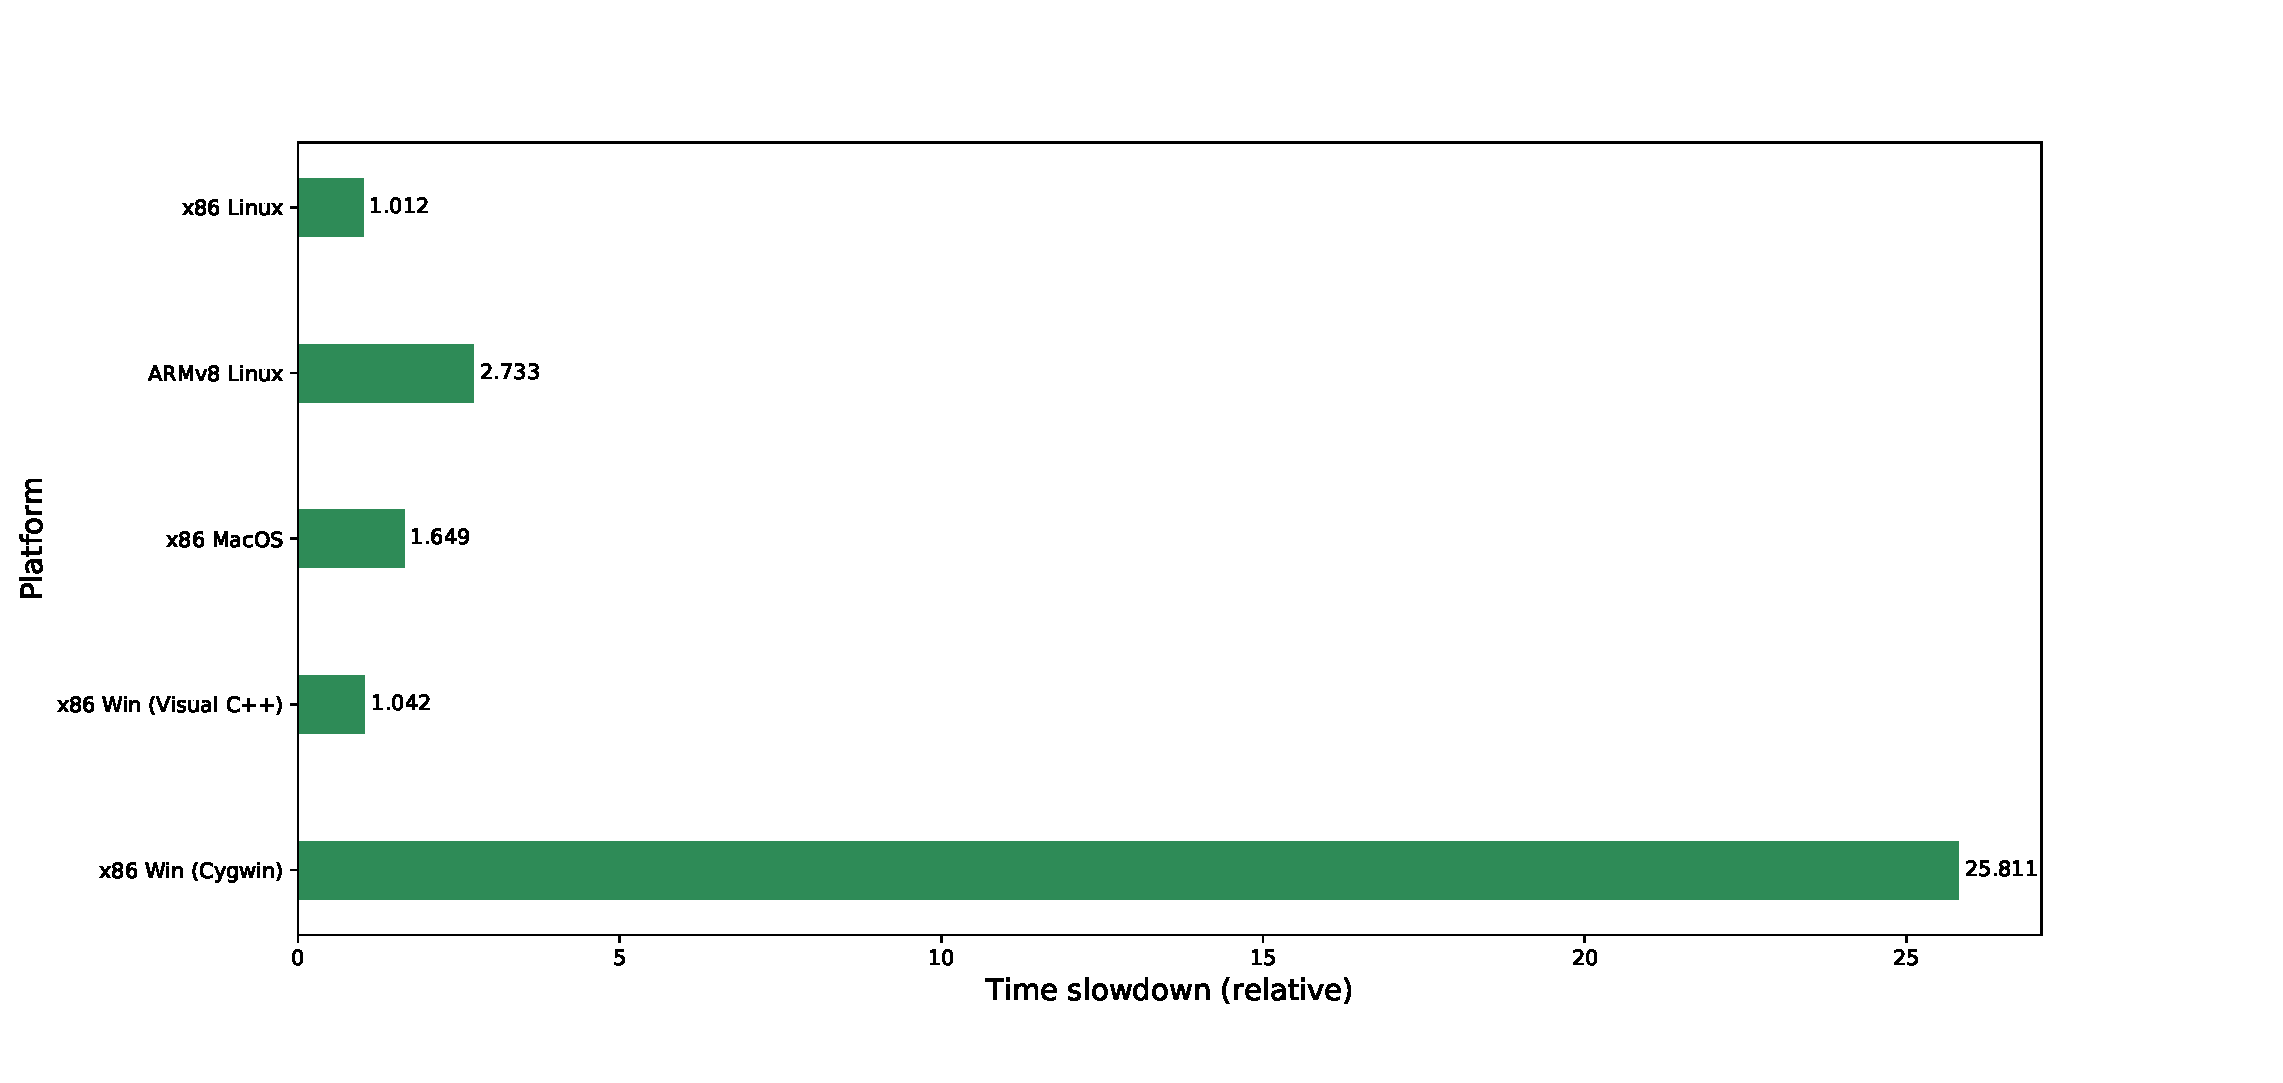
\includegraphics[width=1\linewidth]{thread_local.eps}
\caption{Thread local performance on different platforms (lower is better).}
\label{fig:threadlocal}
\end{figure}

\chapter{Conclusion}
I have successfully implemented a parallel programming language. The language ParVSL
allows the user to employ multi-threading to speed up their algorithms. It offers
a simple shared memory model, based on mutual exclusion and condition variables,
without compromising on any features of the original language VSL. I have demonstrated
this by using it to build a large software project: the REDUCE Algebra System.
I then used it to implement a thread pool and tested it on parallel algorithms with
inter-thread communication, proving a large performance gain can be obtained.

Ultimately, I have shown that a Computer Algebra System can benefit from parallelism,
and have proved that it is possible to modify REDUCE, a large real-world application,
to employ multi-threading effectively. Developers of REDUCE are now able to
use ParVSL to test parallel versions of their algorithms, and some of these developers
have already started testing my system on their workflows.

\section{Lessons learned}

\subsection{Debugging multi-threaded code}

Retrofitting multi-threading into a system designed without parallelism in mind is bound to bring issues.
Many assumptions in original code were violated when running multiple threads. To find and fix all the issues
I had to thoroughly understand every part of the system, which took time.
Sometimes my changes exposed an interaction with some area of code
I had not yet analysed, causing unexpected bugs.

Multi-threaded code is non-deterministic
by nature so many issues would only show up in testing some times when the threads would conflict in just the
right way. Tested behaviour was not always reproducible,
meaning sometimes I only discovered a few bugs weeks after producing them,
when tests which had been passing suddenly failed. making debugging difficult.

Having a large system such as REDUCE provided a great set of regression
tests. However, oftentimes errors showed up after running thousand of lines
of code. This was also code in a language (RLISP) running on top
of a language (LISP) running on top of a third language (C++), so the call stacks
generated were generally unhelpful.

\subsection{Cross platform performance}

Historically, one of the biggest difficulties of implementing multi-threaded languages
was providing cross platform support. I have tested ParVSL on the major platforms and
showed that is capable of supporting them. However, I also discovered that performance
across platforms is very inconsistent. System specific mechanisms of thread local storage
and mutual exclusion have very different implementations and characteristics. This meant
I could not replicate the performance achieved on Linux on other platforms. As of today,
an understanding of each system and careful programming of individual scenarios is still
necessary.

\subsection{Parallelism is hindered by imperative programming}

I discovered that the REDUCE Lisp language included a few historical design decisions which
limit the potential of parallelism, namely its side-effectful nature. The functional programming
paradigm makes it much easier to write safe high-performance multi-threaded programs by avoiding
data races. When using an imperative style, the language has to do extra work to maintain safety,
such as using mutual exclusion on variable access, which can severely slow down any algorithm.

RLisp already offers many features for functional programming.
Modifying REDUCE to avoid side-effectful features of the language, and using a more
functional approach (e.g. avoiding the use of global symbols or the modification
of lists in place) would be needed for it to make good use of multi-threading.

\section{Future work}

While ParVSL is able to support all of REDUCE, it is an interpreted language
which limits its performance. A large number of optimisations are unavailable in this
case and many checks are performed real-time, rather than statically, slowing it down.
The next step would be to use use the lessons learned to modify VSL's brother: CSL.
CSL is compiled and faster than VSL, however it has a much larger code base.
While it would take more work, most of the lessons from writing ParVSL could be translated
to create a similar ParCSL.

The maintainers of REDUCE packages are now able to implement parallel algorithms
for computer algebra, as I have demonstrated with my implementation of
a parallel Buchberger's algorithm for computing Gröbner bases. I showed that
we can achieve speed-ups of over 100\% and it would be interesting to take
this further and evaluate other multi-threaded algorithms described in literature.

While I have focused on the implementation of the Lisp system, I did not formally define
the semantics of the new features. I talked about the trade-offs between safety and performance,
and these need to be carefully considered when establishing the set of guarantees to
provide for multi-threaded programs.

% Bibliography and Appendix
%=============================================================

\addcontentsline{toc}{chapter}{Bibliography}
\printbibliography

\appendix

% \chapter{Glossary}
% \chapter{Glossary of technical terms}


% @@@@@ incomplete




\chapter{Source Code Listings}
\section{Cheney's algorithm}
\label{sec:cheneycode}

\begin{verbatim}
// LispObject is just a pointer type
typedef uintptr_t LispObject;

// LispObject is a pointer type
uintptr_t fringe1, limit1; // heap1, where all allocations happen
uintptr_t fringe2, limit2; // heap2 used for copying GC

LispObject allocate(size_t size) {
  if (fringe1 + size > limit1) {
    collect();
  }

  if (fringe1 + size > limit1) {
     // We are out of memory. Try to increase memory
     // ...
  }

  uintptr_t result = fringe1;
  fringe1 += size;
  return result;
}

// Two helper functions are needed
LispObject copy(LispObject obj) {
  size_t len = size(obj);

  LispObject new_obj = static_cast<LispObject>(fringe2);
  fringe2 += len;
  return new_obj;
}

uintptr_t copycontent(LispObject obj) {
  for (auto ref&: forward_references(obj)) {
    ref = copy(ref);
  }

  return static_cast<uintptr_t>(obj) + size(obj);
}

void collect() {
  // First we copy over the root set, which includes symbols.
  for (LispObject& symbol: symbols_table) {
    symbol = copy(symbol);
  }

  uintptr_t s = heap2;
  while (fringe2 < fringe2) {
    s = copycontent(static_cast<LispObject>(s));
  }

  swap(fringe1, fringe2);
  swap(limit1, limit2);
}
\end{verbatim}

\section{\texttt{Gc\_guard} and \texttt{Gc\_lock}}
\label{sec:gclock-code}

\begin{verbatim}

\end{verbatim}

\section{Lock free symbol lookup}
\label{sec:lockfree-code}
\section{Thread pool}
\label{sec:threadpool-code}

\begin{verbatim}
  lisp;

  symbolic procedure queue;
      {nil, nil};

  symbolic procedure q_push(q, x);
      begin scalar back, newback;
          back := second q;
          newback := {x};

          if null back then <<
              rplaca(q, newback);
              rplaca(cdr q, newback); >>
          else <<
              rplacd(back, newback);
              rplaca(cdr q, newback); >>;
          return q;
      end;

  symbolic procedure q_pop(q);
      begin scalar front, next;
          front := first q;
          if null front then
              return {}
          else <<
              next := cdr front;
              if null next then rplaca(cdr q, {});
              rplaca(q, next);
              return (first front); >>;
      end;

  symbolic procedure q_empty(q);
      null (first q);

  symbolic procedure atomic(val);
      {mutex(), val};

  symbolic procedure atomic_set(a, val);
  begin
      scalar m;
      m := first a;

      mutexlock m;
      rplaca(cdr a, val);
      mutexunlock m;
  end;

  symbolic procedure atomic_get(a);
  begin
      scalar m, res;
      m := first a;

      mutexlock m;
      res := cadr a;
      mutexunlock m;
      return res;
  end;

  symbolic procedure safeq();
      {queue(), mutex(), condvar()};

  symbolic procedure safeq_push(sq, x);
      begin scalar q, m, cv;
          q := first sq;
          m := second sq;
          cv := third sq;

          % print "safeq push getting mutex";
          mutexlock m;
          % print "safeq push got mutex";
          q_push(q, x);
          condvar_notify_one cv;
          % print "safeq push unlocking mutex";
          mutexunlock m;
          return sq;
      end;

  symbolic procedure safeq_pop(sq);
      begin scalar q, m, cv, res;
          q := first sq;
          m := second sq;
          cv := third sq;
          res := nil;

          % print "safeq pop getting mutex";
          mutexlock m;
          % print "safeq pop got mutex";
          % print thread_id ();
          while q_empty q do condvar_wait(cv, m);
          res := q_pop q;
          % print "safeq pop unlocking mutex";
          mutexunlock m;
          % print "safeq pop done";
          return res;
      end;

  % non-blocking call
  symbolic procedure safeq_trypop(sq);
      begin scalar q, m, cv, res;
          q := first sq;
          m := second sq;
          cv := third sq;
          res := nil;

          % print "safeq trypop getting mutex";
          mutexlock m;
          % print "safeq trypop got mutex";

          if q_empty q then
              res := nil
          else
              res := {q_pop q};

          % print "safeq trypop unlocking mutex";
          mutexunlock m;
          return res;
      end;

  symbolic procedure safeq_empty(sq);
      begin scalar r, m;
          m := second sq;
          % print "safeq empty getting mutex";
          mutexlock m;
          % print "safeq empty got mutex";
          r := q_empty (first sq);
          mutexunlock m;
          return r;
      end;

  symbolic procedure future();
      {mutex (), nil};

  % blocking call to wait for future result
  symbolic procedure future_get(fut);
  begin
      scalar m, state, cv, res;
      m := first fut;
      % print "future get getting mutex";
      mutexlock m;
      % print "future get got mutex";

      state := second fut;

      if state = 'done then <<
          res := third fut;
          mutexunlock m;
          return res >>;

      if state = 'waiting then
          cv := third fut
      else <<
          cv := condvar ();
          rplacd(fut, {'waiting, cv}) >>;

      % print "future waiting cv";
      condvar_wait(cv, m);
      % print "future got signaled cv";
      % ASSERT: promise is fulfilled here

      res := third fut;
      % print "future get unlocking mutex";
      mutexunlock m;

      return res;
  end;

  % non-blocking call for future result
  % can wait on cv until timeout
  symbolic procedure future_tryget(fut, timeout);
  begin
      scalar m, state, cv, res;
      m := first fut;
      % print "future tryget getting mutex";
      mutexlock m;
      % print "future tryget got mutex";

      state := second fut;

      if state = 'done then
          res := {third fut}
      else if timeout = 0 then
          res := nil
      else <<
          if state = 'waiting then
              cv := third fut
          else <<
              cv := condvar ();
              rplacd(fut, {'waiting, cv}) >>;

          if condvar_wait_for(cv, m, timeout) then
              res := {third fut}
          else
              res := nil >>;

      % print "future tryget unlocking mutex";
      mutexunlock m;

      return res;
  end;

  symbolic procedure future_set(fut, value);
  begin
      scalar m, state;
      m := first fut;

      % print "future set getting mutex";
      mutexlock m;
      % print "future set got mutex";
      state := second fut;

      if state = 'done then
          error("future already set");

      if state = 'waiting then
          condvar_notify_all third fut;

      rplacd(fut, {'done, value});

      % print "future set unlocking mutex";
      mutexunlock m;
  end;

  symbolic procedure tp_runjob(tp);
  begin
      scalar tp_q, job, resfut, f, args, res;
      tp_q := first tp;
      job := safeq_trypop tp_q;
      if null job then thread_yield ()
      else <<
          job := first job;
          resfut := first job;
          f := second job;
          args := third job;
          res := errorset({'apply, mkquote f, mkquote args}, t);
          future_set(resfut, res);
          % print "done job"
      >>
  end;

  symbolic procedure thread_pool_job(tp_q, status);
  begin
      scalar job, resfut, f, args, res, stat;
      % print "Started worker";
      job := safeq_trypop tp_q;
      repeat <<
          if job then <<
              % print "got job";
              job := first job;
              resfut := first job;
              f := second job;
              args := third job;
              % res := apply(f, args);
              res := errorset({'apply, mkquote f, mkquote args}, t);
              future_set(resfut, res);
              % print "done job";
          >> else <<
              % print "yielding";
              thread_yield ();
          >>;
          job := safeq_trypop tp_q;
          stat := atomic_get status;
      >> until (stat = 'kill) or (stat = 'stop and null job);
      % print "shutting down thread_pool worker";

      return nil
  end;

  symbolic procedure thread_pool(numthreads);
      begin scalar tp_q, status, threads;
          tp_q := safeq();
          status := atomic 'run;
          threads := {};
          % print "starting workers";
          for i := 1:numthreads do threads := thread2('thread_pool_job, {tp_q, status}) . threads;
          return {tp_q, status, threads};
      end;

  symbolic procedure tp_addjob(tp, f, args);
  begin
      scalar tp_q, status, resfut;
      tp_q := first tp;
      status := atomic_get (second tp);

      if not (status = 'run) then
          return nil
      else <<
          resfut := future ();
          % print "pushing job";
          safeq_push(tp_q, {resfut, f, args});
          return resfut;
      >>;
  end;

  symbolic procedure tp_stop(tp);
  begin
      scalar threads;
      % print "tp_stop";
      atomic_set(second tp, 'stop);
      % print "atomic set";
      threads := third tp;
      for each td in threads do <<
          % print "joining thread"; print td;
          jointhread td;
          % print "joined thread";
      >>;
      % print "tp stopped";
      return nil;
  end;

  symbolic procedure tp_kill(tp);
  begin
      scalar threads;
      atomic_set(second tp, 'kill);
      threads := third tp;
      for each td in threads do <<
          % print "joining thread"; print td;
          jointhread td;
          % print "joined thread";
      >>;
  end;

  % tp := thread_pool();

  end;
\end{verbatim}

\chapter{Project Proposal}
% Note: this file can be compiled on its own, but is also included by
% diss.tex (using the docmute.sty package to ignore the preamble)
\documentclass[12pt,a4paper,twoside]{article}
\usepackage[pdfborder={0 0 0}]{hyperref}
\usepackage[margin=25mm]{geometry}
\usepackage{graphicx}
\usepackage{parskip}
\begin{document}
	
	\begin{center}
		\Large
		Computer Science Tripos -- Part II -- Project Proposal\\[4mm]
		\LARGE
		Implementing Parallelism in Lisp for REDUCE
		
		\large
		Andrei-Vlad Badelita, Trinity College
		
		Originator: Dr Arthur C. Norman
		
		15 October 2018
	\end{center}
	
	\vspace{5mm}
	
	\textbf{Project Supervisor:} Dr Arthur C. Norman
	
	\textbf{Directors of Studies:} Prof. Frank Stajano, Dr. Arthur Norman 
	
	\textbf{Project Overseers:} Prof. Jean Bacon, Prof. Ross Anderson, Dr. Amanda Prorok
	
	% Main document
	
	\section*{Introduction}
	
	Computer Algebra System (CAS) programs provide utilities for manipulating mathematical expressions 
	spanning many fields. They employ  numerical algorithms to enable symbolic computations
	on objects such as polynomials or matrices.
	
	Numerical algorithms have long been considered as good candidates for parallel algorithms.
	Oftentimes, the algorithms involve a large number of simple calculations or searching through
	many solutions.
	
	Among the main currently available CAS applications, two are proprietary (Mathematica and Magma),
	while the three main open-source ones (Maxima, Axiom and Reduce) are all written on top of Lisp
	kernels which lack multi-threading support. This is most likely because they have all originally been
	written over thirty years ago, long before the appearance of multi-core personal computers.
	
	Modern computers almost universally provide multiple processing cores, enabling parallelism.
	Moreover, while core counts are increasing, per-core performance improvements have slowed down.
	
	The aim of this project is to prototype multi-threading support for REDUCE. The work would involve
	modifying a smaller Lisp implementation (VSL), which has been used as a development playground
	before for techniques later introduced in the much larger kernel (CSL) that REDUCE normally uses.
	VSL is slower than CSL, but is more compact and manageable. It provides 
	most of the features required to run all of REDUCE, while being fast enough to try
	interesting calculations.
	
	I will augment this code in C++11,  making it
	relatively easy to keep cross-platform compatibility. The current
	code will require modifications to ensure it is thread-safe,
	the garbage collector being a particularly interesting case.
	The language will use a shared memory model with mutexes and signals.
	I will attempt to make these modifications without adding a
	noticeable overhead to existing sequential code, using the current
	REDUCE tests as regression tests and benchmarks. Then I will rewrite
	a few of the numerical algorithms that are inherently parallelisable
	and perform further testing to assess the improvements in performance.
	
	\section*{Starting point}
	
	The REDUCE Computer Algebra System 
	is a long-standing open-source
	project, for which Dr. Arthur Norman is a maintainer. REDUCE runs on a
	LISP back-end, which I am going to modify.
	
	VSL,  the LISP language I am basing my work on, consists of around 4000 lines of
	C code. This code is not written with multi-threading support in mind. C++11 provides good support for multi-threading, which I will make heavy use of.
	
	The REDUCE project comes with a suite of tests. I will use these as regression tests,
	however I will make modifications and add my own during evaluation to test
	the multi-threading component, and assess performance trade-offs.
	
	\section*{Resources required}
	
	I will mainly use my personal laptop, which has a quad-core x86 CPU
	and 16GB of RAM, running Arch Linux. This will be enough to write the code, compile and evaluate.
	Eventually, I might test the compiler on different platforms(Windows, MacOS) and perhaps
	different architectures (e.g. RaspberryPi). I am able to provide all these resources myself. 
	
	I will use version control (Git) to manage both the project and the dissertation, uploading
	to an online mirror (GitHub). I will always keep both a local copy and a cloud-hosted one of the 
	last version of my work. I will make regular backups on removable storage.
	
	I will use the MCS service machine only to upload the project.
	
	\section*{Work to be done}
	
	The project breaks down into the following:
	
	\begin{enumerate}
		
		\item Modifying the existing code to ensure thread-safety.
		
		\item Changing the garbage collector to support safe allocation and
		collection on multiple threads,
		
		\item Implementing the necessary threading primitives: create thread and
		wait for thread, atomics, mutexes, conditional variables, etc.  These will be built on top
		of the their C++11 equivalents.
		
		\item Reimplementing some REDUCE numerical algorithms to benefit from parallelism.
		
	\end{enumerate}
	
	\section*{Success criteria}
	
	The project will be a success if the multi-threaded LISP language is functional,
	running both sequential and parallel code as expected.
	
	To evaluate this, I will first test the storage allocation and garbage
	collection systems. This can be done reasonably early by writing a C++ framework
	to generate patterns of allocation and release of data. By calling  internal
	functions directly, I can assess the validity and performance of the
	garbage collector.
	
	When the entire compiler reaches a working state, I will start writing tests
	in Lisp. These tests will involve common examples of concurrency, such as a
	work queue used by multiple threads.
	
	Finally, running REDUCE and passing the regression tests successfully is
	important. Eventually, I will attempt to extend REDUCE code to make use
	of multi-threading support. Vector and matrix operations are good candidates
	for this.
	
	\section*{Possible extensions}
	
	Once the language is fully functional, I can continue to investigate REDUCE
	algorithms that benefit from the new features. There are two interesting
	algorithms which I can improve:
	
	\begin{itemize}
		\item Polynomial factorisation involves a combinatorial search stage at the
		end, which has the worst potential cost of the entire algorithm. It is a
		well-known bottleneck and could benefit from parallelisation.
		\item Groebner bases represent a case of critical-pair/completion precessing
		for working with ideals generated by multiple polynomial constraints.
		The worst-case cost can be double exponential. Research and other
		implementations in the field show that parallel search can give huge
		performance boosts.
		
	\end{itemize}
	
	Further optimisations of the language can be considered, both in terms of
	performance gains and also difficulty to implement.
	As an example, the current language is interpreted. Given enough time,
	it could be modified to support compilation, which would lead to better performance.
	
	\section*{Timetable}
	
	I have split the timetable in ten work-packages, including eight fortnights and the two
	vacations. The longer vacation breaks will account for break time, and exam preparation,
	however they should still allow a minimum of three weeks of work on the project.
	
	The workload is skewed towards the first few packets. This is meant to allow for extra
	flexibility in the latter part to deal with any particularly difficult aspects of the project.
	
	Planned starting date is Thursday 18/10/2018.
	
	\begin{enumerate}
		
		\item \textbf{Michaelmas weeks 3--4 (18/10/18 -- 31/10/18):} \\ 
		\textbf{DEADLINE 19/10/18:} Submission of final Project Proposal(this document). \\
		Learn to use the LISP implementation. Understand the structure of the compiler code.
		Setup a working build with regression tests. Start identifying thread-unsafe code and
		modifying it.
		
		\item \textbf{Michaelmas weeks 5--6 (01/11/18 -- 14/11/18):} \\
		Reimplement the Garbage Collector to support allocation from multiple threads.
		Ensure single-threaded behaviour is not affected.
		
		\item \textbf{Michaelmas weeks 7--8 (15/11/18 -- 28/11/18):} \\
		Implement functions for multi-threading. Enable creation of threads. Write simple
		tests to show it works. Further work on garbage collector.
		
		\item \textbf{Michaelmas vacation (29/11/18 -- 16/01/19):} \\
		Implement primitives, such as mutexes and condition variables. Analyse the code to
		make sure it is thread safe. Have a working compiler.
		
		\item \textbf{Lent weeks 1--2 (17/01/19 -- 30/01/19):} \\
		Run REDUCE on new compiler and analyse performance trade-off on sequential code.
		Work on progress report and presentation.
		
		\item \textbf{Lent weeks 3--4 (31/01/19 -- 13/02/19):} \\
		\textbf{DEADLINE 01/02/19:} Submission of final Progress Report. \\
		\textbf{07/02/19 -- 12/02/19:} Progress Report Presentations. \\
		Work 
		
		\item \textbf{Lent weeks 5--6 (14/02/19 -- 27/02/19):} \\
		Read about numerical algorithms used inside REDUCE and find
		good examples which benefit from parallelism.
		
		\item \textbf{Lent weeks 7--8 (28/02/19 -- 13/03/19):} \\
		Implement multi-threaded versions of numerical algorithms and
		evaluate performance gain.
		
		\item \textbf{Easter vacation (14/03/19 -- 24/04/19):} \\
		Further evaluation of project. Final improvements to the compiler.
		Write the main chapters of the dissertation.
		
		\item \textbf{Easter term 1--3 (25/04/19 -- 15/05/19):}  \\
		Further evaluation and completion of dissertation.
		
		\textbf{DEADLINE 17/05/19:} Submission of final Dissertation. \\
		
	\end{enumerate}
	
\end{document}


\end{document}
